\documentclass[letterpaper, peerreview, draftcls]{IEEEtran}
%
% If IEEEtran.cls has not been installed into the LaTeX system files,
% manually specify the path to it like:
% \documentclass[journal]{../sty/IEEEtran}

% *** CITATION PACKAGES ***
%
\usepackage{cite}
\usepackage[hidelinks]{hyperref}
% cite.sty was written by Donald Arseneau
% V1.6 and later of IEEEtran pre-defines the format of the cite.sty package
%\cite{} output to follow that of the IEEE. Loading the cite package will
% result in citation numbers being automatically sorted and properly
% 'compressed/ranged'. e.g., [1], [9], [2], [7], [5], [6] without using
% cite.sty will become [1], [2], [5]--[7], [9] using cite.sty. cite.sty's
%\cite will automatically add leading space, if needed. Use cite.sty's
% noadjust option (cite.sty V3.8 and later) if you want to turn this off
% such as if a citation ever needs to be enclosed in parenthesis.
% cite.sty is already installed on most LaTeX systems. Be sure and use
% version 5.0 (2009-03-20) and later if using hyperref.sty.
% The latest version can be obtained at:
% http://www.ctan.org/pkg/cite
% The documentation is contained in the cite.sty file itself.

% *** GRAPHICS RELATED PACKAGES ***
%
\ifCLASSINFOpdf{}
  \usepackage[pdftex]{graphicx}
  % declare the path(s) where your graphic files are
  \graphicspath{{./pdf/}{./jpg/}}
  % and their extensions so you won't have to specify these with
  % every instance of \includegraphics
  \DeclareGraphicsExtensions{.pdf,.jpg,.png}
\else
  % or other class option (dvipsone, dvipdf, if not using dvips). graphicx
  % will default to the driver specified in the system graphics.cfg if no
  % driver is specified.
  % \usepackage[dvips]{graphicx}
  % declare the path(s) where your graphic files are
  % \graphicspath{{../eps/}}
  % and their extensions so you won't have to specify these with
  % every instance of \includegraphics
  % \DeclareGraphicsExtensions{.eps}
\fi

% *** MATH PACKAGES ***
%
\usepackage{amsmath}
\newcommand*\mean[1]{\bar{#1}}
% A popular package from the American Mathematical Society that provides
% many useful and powerful commands for dealing with mathematics.

% *** SPECIALIZED LIST PACKAGES ***

% *** ALIGNMENT PACKAGES ***
%
%\usepackage{array}
% Frank Mittelbach's and David Carlisle's array.sty patches and improves
% the standard LaTeX2e array and tabular environments to provide better
% appearance and additional user controls. As the default LaTeX2e table
% generation code is lacking to the point of almost being broken with
% respect to the quality of the end results, all users are strongly
% advised to use an enhanced (at the very least that provided by array.sty)
% set of table tools. array.sty is already installed on most systems. The
% latest version and documentation can be obtained at:
% http://www.ctan.org/pkg/array

% IEEEtran contains the IEEEeqnarray family of commands that can be used to
% generate multiline equations as well as matrices, tables, etc., of high
% quality.

% *** SUBFIGURE PACKAGES ***
\ifCLASSOPTIONcompsoc
 \usepackage[caption=false,font=normalsize,labelfont=sf,textfont=sf]{subfig}
\else
 \usepackage[caption=false,font=footnotesize]{subfig}
\fi

% *** FLOAT PACKAGES ***

% *** PDF, URL AND HYPERLINK PACKAGES ***
%
\usepackage{url}

% correct bad hyphenation here
\hyphenation{op-tical net-works semi-conduc-tor}

\usepackage[nolist]{acronym}

\usepackage{tabularx}
\usepackage{booktabs}
\usepackage{multirow}
\usepackage{adjustbox}

% line breaks in table cells
\newcommand{\specialcell}[2][l]{%
  \begin{tabular}[#1]{@{}l@{}}#2\end{tabular}}

\usepackage{xtab}

\usepackage{csquotes}

\usepackage[utf8]{inputenc}
% enables custom font styles which are not available in IEEEtran by default
% https://tex.stackexchange.com/questions/331228/there-is-no-bold-text-italics-in-ieeetran

\renewcommand{\sfdefault}{cmss}
\renewcommand{\rmdefault}{cmr}
\renewcommand{\ttdefault}{cmt}

\usepackage[detect-all]{siunitx}

\begin{document}
%
% paper title
% Titles are generally capitalized except for words such as a, an, and, as,
% at, but, by, for, in, nor, of, on, or, the, to and up, which are usually
% not capitalized unless they are the first or last word of the title.
% Linebreaks \\ can be used within to get better formatting as desired.
% Do not put math or special symbols in the title.
\title{Monitoring forest health using hyperspectral imagery: Does feature selection improve the performance of machine-learning techniques?}
\IEEEpeerreviewmaketitle{Monitoring forest health using hyperspectral imagery: Does feature selection improve the performance of machine-learning techniques?}
%
%
% author names and IEEE memberships
% note positions of commas and non-breaking spaces ( ~ ) LaTeX will not break
% a structure at a ~ so this keeps an author's name from being broken across
% two lines.
% use \thanks{} to gain access to the first footnote area
% a separate \thanks must be used for each paragraph as LaTeX2e's \thanks
% was not built to handle multiple paragraphs
%

% suppress 'underfull hbox' warnings
\hbadness=99999

\author{Patrick~Schratz,
	Jannes~Muenchow,
	Eugenia~Iturritxa,
	José~Cortés,
	Bernd~Bischl,
	and Alexander~Brenning
	\thanks{P.Schratz, J.Muenchow, J.Cortés and A.Brenning are with the Department
		of Geography, GIScience group, Friedrich-Schiller-University of Jena, Germany.}% <-this % stops a space
	\thanks{B.Bischl is head of the computational statistics group at the Department of Statistics, Ludwig-Maximilian-University Munich.}% <-this % stops a space
	\thanks{E.Iturritxa is with NEIKER Tecnalia, Vitoria-Gasteiz, Arab, Spain.}% <-this % stops a space
	%\thanks{Manuscript received April 19, 2005; revised August 26, 2015.}
}

% note the % following the last \IEEEmembership and also \thanks -
% these prevent an unwanted space from occurring between the last author name
% and the end of the author line. i.e., if you had this:
%
% \author{....lastname \thanks{...} \thanks{...} }
%                     ^------------^------------^----Do not want these spaces!
%
% a space would be appended to the last name and could cause every name on that
% line to be shifted left slightly. This is one of those 'LaTeX things'. For
% instance, '\textbf{A} \textbf{B}' will typeset as 'A B' not 'AB'. To get
% 'AB' then you have to do: '\textbf{A}\textbf{B}'
% \thanks is no different in this regard, so shield the last } of each \thanks
% that ends a line with a % and do not let a space in before the next \thanks.
% Spaces after \IEEEmembership other than the last one are OK (and needed) as
% you are supposed to have spaces between the names. For what it is worth,
% this is a minor point as most people would not even notice if the said evil
% space somehow managed to creep in.

% The paper headers
\markboth{IEEE Transactions on Geoscience and Remote Sensing}%
{Shell \MakeLowercase{\textit{et al.}}: Bare Demo of IEEEtran.cls for IEEE Journals}
% The only time the second header will appear is for the odd numbered pages
% after the title page when using the twoside option.
%
% *** Note that you probably will NOT want to include the author's ***
% *** name in the headers of peer review papers.                   ***
% You can use \ifCLASSOPTIONpeerreview for conditional compilation here if
% you desire.

% make the title area
\maketitle

% As a general rule, do not put math, special symbols or citations
% in the abstract or keywords.
\begin{abstract}
	This study analyzed highly-correlated, feature-rich datasets from hyperspectral remote sensing data using multiple machine and statistical-learning methods.
	The effect of filter-based feature-selection methods on predictive performance was compared.
	Also, the effect of multiple expert-based and data-driven feature sets, derived from the reflectance data, was investigated.
	Defoliation of trees (\%) was modeled as a function of reflectance, and variable importance was assessed using permutation-based feature importance.
	Overall support vector machine (SVM) outperformed others such as random forest (RF), extreme gradient boosting (XGBoost), lasso (L1) and ridge (L2) regression by at least three percentage points.
	The combination of certain feature sets showed small increases in predictive performance while no substantial differences between individual feature sets were observed.
	For some combinations of learners and feature sets, filter methods achieved better predictive performances than the unfiltered feature sets, while ensemble filters did not have a substantial impact on performance.

	Permutation-based feature importance estimated features around the red edge to be most important for the models.
	However, the presence of features in the near-infrared region (800 nm - 1000 nm) was essential to achieve the best performances.

	More training data and replication in similar benchmarking studies is needed for more generalizable conclusions.
	Filter methods have the potential to be helpful in high-dimensional situations and are able to improve the interpretation of feature effects in fitted models, which is an essential constraint in environmental modeling studies.

\end{abstract}

% Note that keywords are not normally used for peer-review papers.
\begin{IEEEkeywords}
	hyperspectral imagery, forest health monitoring, machine learning, feature selection, feature effects, model comparison
\end{IEEEkeywords}

% For peer-review papers, this IEEEtran command inserts a page break and
% creates the second title. It will be ignored for other modes.
\IEEEpeerreviewmaketitle{}

\renewcommand{\IEEEiedlistdecl}{\IEEEsetlabelwidth{SONET}}
\begin{acronym}

	% geringerer Zeilenabstand

	%\setlength{\itemsep}{-\parsep}
	\acro{AGB}{above-ground biomass}
	\acro{ALE}{accumulated local effects}
	\acro{ALS}{airborne laser scanning}
	\acro{ANN}{artificial neural network}
	\acro{AUROC}{area under the receiver operating characteristics curve}
	\acro{BRT}{boosted regression trees}
	\acro{CART}{classification and regression trees}
	\acro{CNN}{convolutional neural networks}
	\acro{CV}{cross-validation}
	\acro{DAP}{digital aerial photogrammetry}
	\acro{ENM}{environmental niche modeling}
	\acro{FPR}{false positive rate}
	\acro{FFS}{forward feature selection}
	\acro{FS}{feature selection}
	\acro{GAM}{generalized additive model}
	\acro{GBM}{gradient boosting machine}
	\acro{GLM}{generalized linear model}
	\acro{ICGC}{Institut Cartografic i Geologic de Catalunya}
	\acro{IQR}{interquartile range}
	\acro{MARS}{multivariate adaptive regression splines}
	\acro{MBO}{model-based optimization}
	\acro{MEM}{maximum entropy model}
	\acro{ML}{machine learning}
	\acro{NDII}{normalized difference infrared index}
	\acro{NIR}{near-infrared}
	\acro{NRI}{normalized ratio index}
	\acro{NDMI}{normalized difference moisture index}
	\acro{OLS}{ordinary least squares}
	\acro{LiDAR}{light detection and ranging}
	\acro{LOWESS}{locally weighted scatter plot smoothing}
	\acro{PISR}{potential incoming solar radiation}
	\acro{PCA}{principal component analysis}
	\acro{PDP}{partial dependence plots}
	\acro{PLS}{partial least-squares}
	\acro{RBF}{radial basis function}
	\acro{RF}{random forest}
	\acro{RMSE}{root mean square error}
	\acro{RR}{ridge regression}
	\acro{RSS}{residual sum of squares}
	\acro{SAR}{synthetic aperture radar}
	\acro{SDM}{species distribution modeling}
	\acro{SMBO}{sequential-based model optimization}
	\acro{SVM}{support vector machine}
	\acro{TPR}{true positive rate}
	\acro{VI}{vegetation index}
	\acro{XGBoost}{extreme gradient boosting}
\end{acronym}
\renewcommand{\IEEEiedlistdecl}{\relax}% reset back

\section{Introduction}
% Explain how remote sensing is used in forestry (potential to map forest health)

% Link remote sensing and machine-learning

\IEEEPARstart{T}{he} use of \ac{ML} algorithms for analyzing remote sensing data has seen a huge increase in the last decade \cite{lary2016}.
Naturally, this coincided with the increased availability of remote sensing imagery, especially since the launch of the first Sentinel satellite in the year 2014.
At the same time, the implementation and usability of learning algorithms has been greatly simplified with many contributions from the open-source community.
Scientists can nowadays process large amounts of (environmental) information with relative ease using various learning algorithms.
This makes it possible to extend the benchmark comparison matrix of studies in a semi-automated way, possibly stumbling across unexpected findings of process settings that would never have been explored otherwise \cite{ma2015}.

% link to forest health analysis and show exemplary studies

Machine-learning methods in combination with remote sensing data are used in many environmental fields such as vegetation cover analysis or forest carbon storage mapping \cite{mascaro2014, urban2018}.
The ability of predicting into unknown space qualifies these tools as a promising toolset for such tasks.
One aspect of this research field is to enhance the understanding of biotic and abiotic stress triggers, for example by analyzing tree defoliation \cite{hawrylo2018}.

Other approaches for analyzing forest health include change detection \cite{zhang2016} or describing the current health status of forests on a stand level \cite{townsend2012}.
In such studies, the defoliation of trees serves as a proxy for forest health by describing the impact of biotic and abiotic pest triggers \cite{townsend2012, goodbody2018}.

Vegetation indices have shown the potential to provide valuable information when analyzing forest health \cite{jiang2014, adamczyk2015}.
Most vegetation indices were developed with the aim of being sensitive to changes of specific wavelength regions, serving as a proxy for underlying plant processes.
However, often enough indices developed for different purposes than the one to be analyzed can help to explain complex relationships.
This emphasizes the need to extract as much information as possible from the available input data to generate promising features which can help to understand the modeled relationship.
A less known index type which can be derived from spectral information is the \ac{NRI}.
In contrast to most vegetation indices, \ac{NRI}s do not use an expert-based formula following environmental heuristics but instead makes use of a data-driven feature engineering approach by combining (all possible) combinations of spectral bands.
Especially when working with hyperspectral data, thousands of \ac{NRI} features can be derived this way.

% now that we introduced the importance of remote sensing indices for forest health,

Despite their popularity in environmental modeling, there are no studies so far which used machine-learning algorithms in combination with remote sensing data to analyze defoliation at the tree level.
This study aims to close this gap by analyzing tree defoliation in northern Spain using airborne hyperspectral data.
The methodology of this study uses machine-learning methods in combination with feature selection and hyperparameter tuning.
In addition, feature importance and feature effects are evaluated.
Incorporating the idea of creating data-driven \ac{NRI}s, this study also discusses the practical problems of high dimensionality in environmental modeling \cite{trunk1979, xu2016}.

% mention why FS is used / important
Even though \ac{ML} algorithms are capable of handling highly correlated input variables, model fitting becomes computationally more demanding, and model interpretation more complex.
Feature selection approaches can help to address this issue, reducing possible noise in the feature space, simplify model interpretability and possibly enhance predictive performance \cite{cai2018}.

% clarify the focus of this study
This study shows how high-dimensional datasets can be handled effectively with machine-learning methods while still being able to interpret the fitted models.
The predictive power of non-linear methods and their ability to handle highly correlated predictors is combined with common and new approaches for assessing feature importance and feature effects.
However, this study clearly focuses on investigating the effects of filter methods and feature set types on predictive performance rather than on interpreting feature effects.

Considering these opportunities and challenges, the research questions of this study are the following:

\begin{itemize}

	\item Do different (environmental) feature sets show differences in performance when modeling defoliation of trees?

	\item Can predictive performance be substantially improved by combining feature sets?

	\item How do different feature selection methods influence the predictive performance of the models?

	\item Which features are most important and how can these be interpreted in an environmental context?

\end{itemize}

\section{Data and study area}

Airborne hyperspectral data with a spatial resolution of one meter and 126 spectral bands was available for four Monterey Pine (\textit{Pinus radiata D. Don}) plantations in northern Spain.
The trees in the plots suffer from infections of invasive pathogens such as \textit{Diplodia sapinea (Fr.) Fuckel}, \textit{Fusarium circinatum Nirenberg \& O'Donnell}, \textit{Armillaria mellea (Vahl) P. Kumm}, \textit{Heterobasidion annosum (Fr.) Bref}, \textit{Lecanosticta acicola (Thüm) Syd.} and \textit{Dothisthroma septosporum (Dorogin) M. Morelet} causing a spread of cankers or defoliation \cite{mesanza2016, iturritxa2017}.
The last two fungi are mainly responsible for the foliation loss of the trees analyzed in this study \cite{iturritxa2014}.
In-situ measurements of defoliation of trees (serving as a proxy for tree health) were collected to serve as the response variable \textit{defoliation} which ranges from 0 - 100 (in \%) (\autoref{fig:defol-distr}).
It is assumed that the fungi infect the trees through open wounds, possibly caused by previous hail damage \cite{iturritxa2014}.
The dieback of these trees, which are mainly used as timber, causes high economic damages \cite{ganley2009}.

\begin{figure} [t!]
	\centering
	\begin{center}
		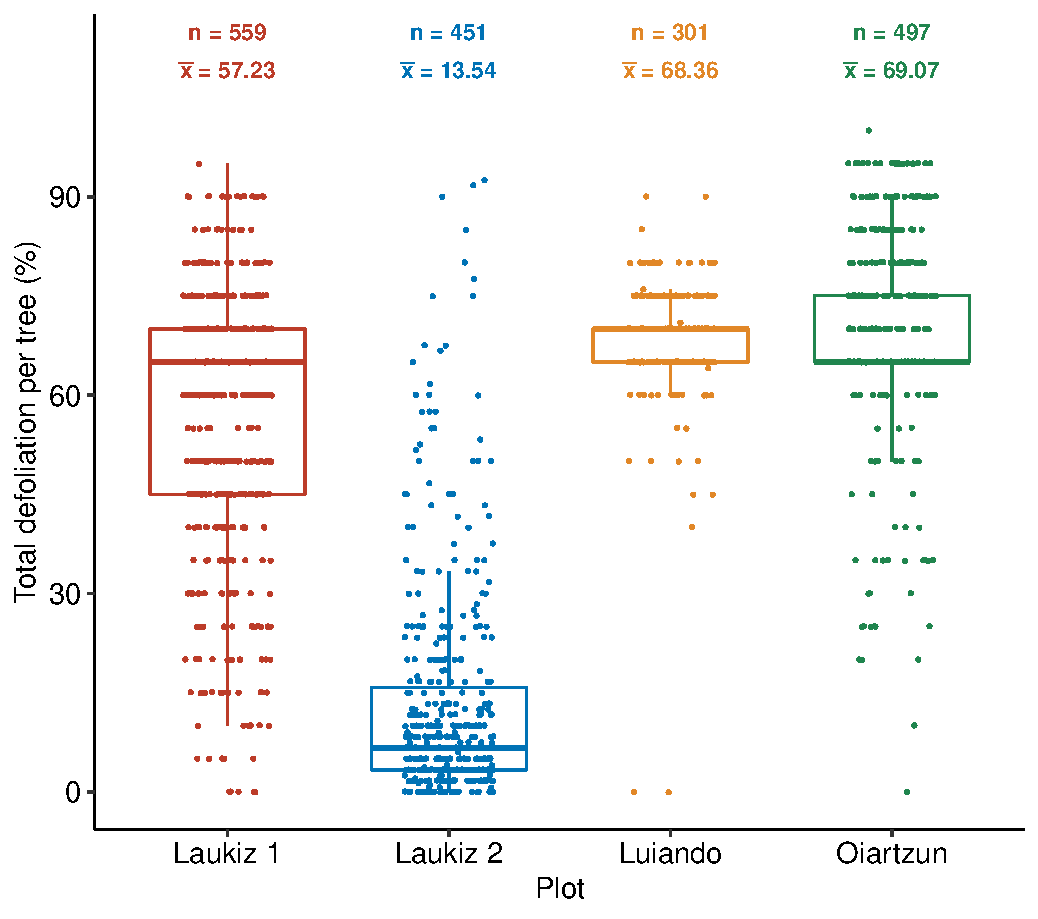
\includegraphics[width=0.48\textwidth] {defoliation-distribution-plot-1.pdf}
		\caption{Response variable \textit{defoliation} at trees for plots Laukiz1, Laukiz2, Luiando and Oiartzun. \texttt{n} corresponds to the total number of trees in the plot, $\bar{x}$ refers to the mean defoliation.}\label{fig:defol-distr}
	\end{center}
\end{figure}

\subsection{In-situ data}

The \textit{Pinus radiata} plots of this study, namely Laukiz1, Laukiz2, Luiando and Oiartzun, are located in the northern part of the Basque Country (\autoref{fig:study_area}).
Oiartzun has the most observations (n = 559) while Laukiz2 shows the largest area size (1.44 ha).
All plots besides Luiando are located within 100 km from the coast (\autoref{fig:study_area}).
In total 1808 observations are available (Laukiz1 = 559, Laukiz2 = 451, Luiando = 301, Oiartzun = 497).
Field surveys were conducted in September 2016.

\begin{figure*} [ht!]
	\begin{center}
		\centering
		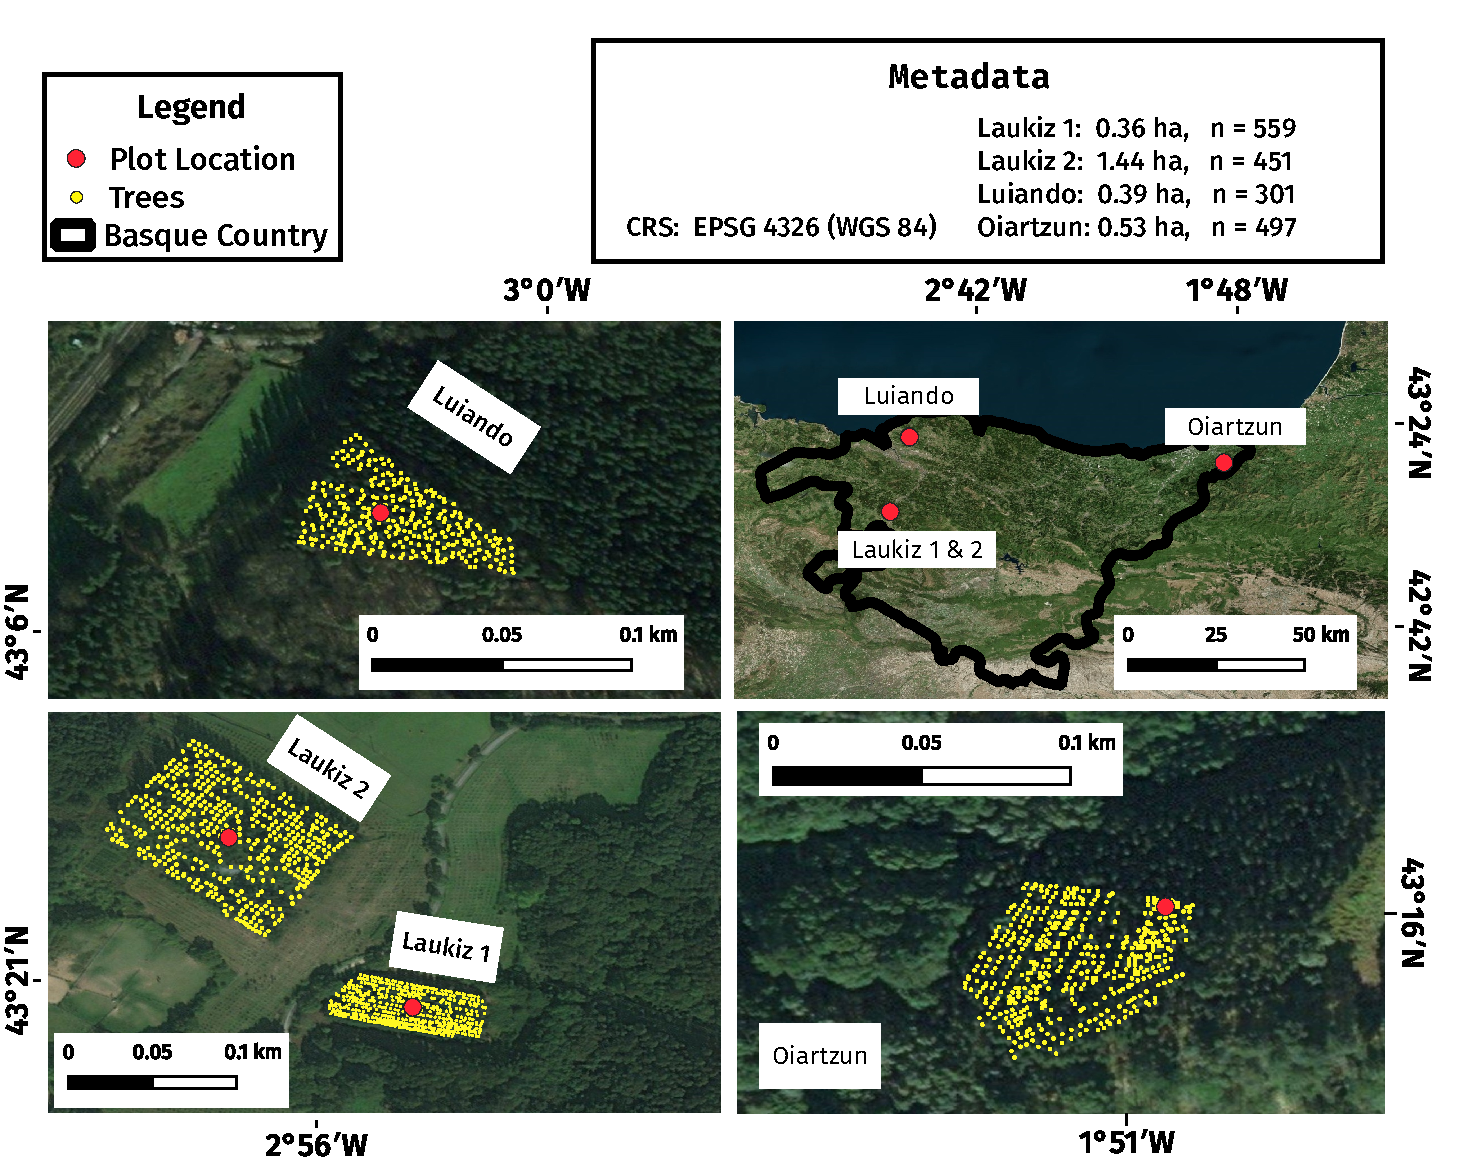
\includegraphics[width=\textwidth] {study-area-hyperspectral.pdf}
		\caption{Information about location, size and spatial distribution of trees for all plots used in this study.}\label{fig:study_area}
	\end{center}
\end{figure*}

%\begin{figure} [t!]
%	\begin{center}
%		\includegraphics[width=0.48\textwidth] {defol-grid-3000px.jpg}
%		\caption{Example trees showing different levels of defoliation as interpreted by the surveyor: 10 \% (top-left), 20 \% (top-right), 40 \% (bottom-left), 60-70 \% (bottom-right).}
%		\label{fig:defol-trees}
%	\end{center}
%\end{figure}

\subsection{Hyperspectral data}

The airborne hyperspectral data was acquired during two flight campaigns which took place at noon on September 28th and October 5th 2016.
The images were taken by an AISAEAGLE-II sensor.
All preprocessing steps (geometric, radiometric, atmospheric) were conducted by the \ac{ICGC}.
The first four bands were corrupted, leaving 122 bands with valid information.
Additional metadata information is available in \autoref{tab:hyperparameter_metadata}.

% parameter limits

\begin{table}[t]
	\centering
	\caption[t]{Specifications of hyperspectral data.}
	\begingroup
	\begin{tabular}{ll}
		\\
		Characteristic         & Value                               \\
		\toprule
		Geometric resolution   & 1 m                                 \\
		Radiometric resolution & 12 bit                              \\
		Spectral resolution    & 126 bands (404.08 nm --- 996.31 nm) \\
		Correction:            & Radiometric, geometric, atmospheric
	\end{tabular}
	\endgroup\label{tab:hyperparameter_metadata}
\end{table}

\section{Methods}

\subsection{Derivation of indices}

To use the full potential of the hyperspectral data, all possible vegetation indices supported by the R package hsdar (89 in total) as well as all possible \ac{NRI} combinations were calculated from the reflectances.
The following formula was used for the NRI calculation:

\begin{equation}
	NRI_{i,j} = \frac{band_{i} - band_{j}}{band_{i} + band_{j}}
\end{equation}

\noindent
with \(i\) and \(j\) being the respective band numbers.

\bigbreak{}

To account for geometric offsets within the hyperspectral data, which were reported with up to 1 m from \ac{ICGC}, a buffer of two meters around the centroid of each tree was used when extracting the reflectance values.
A pixel was considered to fall into a tree's buffer zone if the centroid of the respective pixel was touched by the buffer.
All of those pixels formed the final reflectance value of a single tree and were used as the base information to derive all additional feature sets.
In total, \(\frac{121*122}{2} = 7471\) NRIs were calculated.

\subsection{Feature selection}

High-dimensional, feature-rich datasets come with several challenges for both model fitting and evaluation.

\begin{itemize}
	\item Model fitting times increase.
	\item Noise is possibly introduced into models by highly correlated variables \cite{johnstoneiainm.2009}.
	\item Model interpretation and prediction become more challenging \cite{johnstoneiainm.2009}.
\end{itemize}

To reduce the feature space of a dataset, conceptually differing approaches exist: wrapper methods, filters, penalization methods (lasso and ridge) or \ac{PCA} \cite{bommert2020, das2001, guyon2003, jolliffe2016}.
In contrast to wrapper methods, filters can be added to the hyperparameter optimization step and have a lower computational footprint.
Due to the focus on filter methods in this manuscript, only this sub-group of feature selection methods will be introduced in greater detail in the following subsections.

\subsubsection{Filter methods}

% Filter methods
The concept of filters originates from the idea of ranking features following a score calculated by an algorithm \cite{guyon2003}.
Some filter methods can only deal with specific types of variables (numeric or nominal).
Filters only rank features, they do not decide which covariates to drop or keep \cite{drotar2015}.
The selection which features to keep for model fitting is usually done within the optimization phase of the model fitting, along with the hyperparameter tuning.
Essentially, the number of covariates in the model is treated as a additional hyperparameter of the model.
The goal is to optimize the number of ranked features to the point at which the model achieves the best performance.

% Ensemble filter methods
Besides the concept of choosing a specific filter method to rank variables, studies showed that combining several filters using statistical operations such as 'minimum' or 'mean' can enhance the predictive performance of the resulting models, especially when applied to multiple datasets \cite{abeel2010, drotar2017a}.
This approach is referred to as 'ensemble filtering' \cite{dietterich2000}.
Ensemble filters align with the recent rise of the 'ensemble' approach in machine learning which uses the idea of stacking to combine the predictions of multiple models, aiming to enhance predictive performance \cite{polikar2012, feurer2015, bolon-canedo2019}.
In this work the 'Borda' ensemble filter was applied \cite{drotar2017a}.
Its final feature order is determined by the sum of all single filters ranks.

% Ensuring a fair weighting in the ensemble
Filter methods can be grouped into groups which are formed out of three binary classes: multivariate or univariate feature use, correlation or entropy-based importance weighting and linear and non-linear filter methodology.
Care needs to be taken to not weigh certain classes more than others in the ensemble as otherwise the final ranking result will be biased.
In this study this was taken care of by checking the rank correlations (Spearman's correlation) of the generated feature rankings of all methods against each other.
If filter pairs showed a correlation of 0.9 or higher, only one of the two was included into the ensemble filter, selected at random.
This ensured that the ensemble filter composition was not biased towards a certain group of filter methods.

\subsubsection{Description of used filter methods}

Filter methods can be classified as follows (\autoref{tab:filter-methods}):

\begin{itemize}
	\item Univariate/multivariate (scoring based on a single variable / multiple variables).
	\item Linear/non-linear (usage of linear/non-linear calculations).
	\item Entropy/correlation (scoring based on derivations of entropy or correlation-based approaches).
\end{itemize}

% filter methods
\begin{table}[b!]
	\centering
	\caption{List of filter methods used in this work}
	\label{tab:filter-methods}
	\begingroup\footnotesize
	\begin{adjustbox}{width={0.48\textwidth},totalheight={\textheight},keepaspectratio}
		\begin{tabular}{lll}
			\\
			Name                                         & Group                             & Ref.               \\
			\toprule
			Linear correlation (Pearson)                 & univariate, linear, correlation   & \cite{pearson1901} \\
			Information gain                             & univariate, non-linear, entropy   & \cite{quinlan1986} \\
			Minimum redundancy, maximum relevance        & multivariate, non-linear, entropy & \cite{zhao2013}    \\
			Carscore                                     & multivariate, linear, correlation & \cite{zuber2011}   \\
			Relief                                       & multivariate, linear, entropy     & \cite{kira1992}    \\
			Conditional minimal information maximization & multivariate, linear, entropy     & \cite{fleuret2004}
		\end{tabular}
	\end{adjustbox}
	\endgroup
\end{table}

The filter 'Information Gain' is only defined for nominal response variables:

\begin{equation}
	H(Class) + H(Attribute) - H(Class, Attribute)
\end{equation}

where \(H\) is the conditional entropy of the response variable (class) or the feature (attribute), respectively.
In order to use this method with a numeric response (percentage defoliation of trees), the variable was discretized into equal bins and treated as a class variable.
After feature rank correlations of $> 0.9$ between different bin sizes were observed in a side analysis, \texttt{\(n_{bin}\) = 10} was found to be a reasonable setting to go with.

\subsection{Benchmarking design}

\subsubsection{Algorithms}

The following learners were used in this work:

\begin{itemize}
	\item  Extreme Gradient Boosting (XGBoost)
	\item  Random Forest (RF)
	\item  Penalized Regression (both L1 (lasso) and L2 (ridge))
	\item  Support Vector Machine (SVM, RBF Kernel)
\end{itemize}

Random forest and {SVM} are well established algorithms widely used in (environmental) remote sensing.
Extreme Gradient Boosting (commonly abbreviated as XGBoost) has shown promising results in benchmark studies in recent years.
Penalized regression is a statistical modeling technique capable of dealing with highly-correlated covariates by penalizing the coefficients of the model \cite{hastie2001}.
Common penalties are 'lasso' (L1) and 'ridge' (L2).
Ridge does not remove variables from the model (penalization to zero) but just shrinks them to effectively zero, keeping them in the model.

\subsubsection{Feature sets}

Three feature sets were used in this study, each representing a different approach to feature engineering:

\begin{itemize}
	\item The raw hyperspectral band information (HR): no feature engineering) %chktex 13
	\item Vegetation Indices (\ac{VI}s): expert-based feature engineering)
	\item Normalized Ratio Indices (\ac{NRI}s): data-driven feature engineering)
\end{itemize}

The idea of splitting the features into different sets originated from the question whether feature-engineered indices derived from reflectance values have a positive effect on model performance.
\cite{pena2017} is an exemplary study which used this approach in a spectro-temporal setting.
Benchmarking learners on these feature sets while keeping all other variables such as model type, tuning strategy and partitioning method constant makes it possible to draw conclusions on their individual impact.
However, rather than only looking at these three groups also combinations of such were taken into account:

\begin{itemize}
	\item HR + VI %chktex 13
	\item HR + NRI
	\item HR + VI + NRI
\end{itemize}

Even though the feature-selection step should be solely left to the filter methods in this study, it was ensured a priori to account for features with a pairwise correlation of 1.
Having such features within the data can cause undesired effects during model fitting and feature importance calculation.
Hence, after having calculated all pair-wise correlations between features, for pairs which exceeded the threshold of $1 - 10^{-10}$, the feature with the largest mean absolute correlation across all variables was removed from the dataset.

This preprocessing step reduced the number of covariates to 122 (HR), 86 (VI) and 7467 (NRI).

\subsubsection{Hyperparameter Optimization}

Hyperparameters were tuned using \ac{MBO} within a nested spatial \ac{CV} \cite{mlrmbo, binder2020, schratz2019}.
In MBO first \textit{n} randomly chosen hyperparameter settings out of a user defined search space are composed.
After these \textit{n} settings have been evaluated, one new setting, which is going to be evaluated next, is proposed by a fitted surrogate model (by default a kriging method).
This strategy continues until a termination criterion, defined by the user, is reached \cite{hutter2011, jones1998}.

In this work, an initial design of 30 randomly composed hyperparameter settings in combination with a termination criterion of 70 iterations was used, resulting in a total budget of 100 evaluated hyperparameter settings per fold.
The advantage of this tuning approach is a substantial reduction of the tuning budget that is required to find a setting close to the global optimization minimum.
\ac{MBO} may outperform methods that do not use information from previous iterations, such as random search or grid search \cite{bergstra2012}.

To optimize the number of features used for model fitting, the percentage of features was added as a hyperparameter during the optimization stage (\cite{binder2020}).
For \ac{PCA}, the number of principal components was tuned instead.
%The RF hyperparameter \texttt{\(m_{try}\)} was re-expressed as $m_{try} = p^x_{try}$.
The RF hyperparameter \texttt{\(m_{try}\)} was re-expressed as $m_\textrm{try} = p_\textrm{sel}^t$ as a function of the number of selected features, $p_\textrm{sel}$.
It was thus tuned on a logarithmic scale by varying $t$ between 0 (i.e. $m_\textrm{try} = 1$) and 0.5 (i.e. $m_\textrm{try}=\sqrt{p_\textrm{sel}}$).
This was necessary to ensure that \texttt{\(m_{try}\)} was not chosen higher than the available number of features left after optimizing the feature percentage during tuning.

\subsubsection{Spatial resampling}

A spatial nested cross-validation on the plot level was chosen to reduce the influence of spatial autocorrelation as much as possible \cite{schratz2019, sperrorest}.
The \ac{RMSE} was chosen as the error measure.
Each plot served as one fold within the cross-validation setting, resulting in four iterations in total.
For the inner level (hyperparameter tuning), \(k - 1\) folds were used with \(k\) being the number of plots.

In total the benchmarking grid consisted of 156 experiments (6 feature sets $\times$ 3 ML algorithms $\times$ 8 feature-selection methods and for the L1/L2 models, 6 feature sets $\times$ 2 models.

\subsection{Feature importance and feature effects}

Estimating feature importance for datasets with highly correlated features is a complicated task for which many different approaches, model-specific and agnostic, exist \cite{friedman2001, hastie2001, greenwell2018}.
The correlation between covariates makes it challenging to calculate an unbiased estimate for single features \cite{molnar2019}.
Methods like \ac{PDP} or permutation-based approaches may produce unreliable estimates in such scenarios because unrealistic situations between covariates are created \cite{molnar2019}.
The development of robust methods which enable an unbiased estimation of feature importance for highly correlated variables are subject to current research.

In this work permutation-based feature importance and \ac{ALE} plots (HR only) were calculated to estimate feature importance / effects \cite{apley2019, molnar2019}.
With the limitations of both methods in mind when applied to correlated features, the aim was to get a general overview of the feature importance of the hyperspectral bands while trying to avoid an over-interpretation of results.
The best-performing algorithm on the HR task (i.e. SVM) was used for the feature importance calculation.

\subsection{Linking feature importance to wavelength regions}

For environmental interpretation purposes the ten most important indices of the best performing models of feature sets HR and VI were linked to the spectral regions of the hyperspectral data.
The aim was to visualize the most important features along the spectral curve of the plots to better understand which spectral regions were most important for the model.

\subsection{Research compendium}

All tasks of this study were conducted using the open-source statistical programming language R \cite{rcoreteam2019}.
A complete list of all R packages used in this study can be found in linked repositories.
Due to space limitations only the selected packages with high impact on this work will be explicitly cited.

The algorithm implementations of the following packages have been used: xgboost \cite{chen2016} (\textit{Extreme Gradient Boosting}), kernlab \cite{kernlab} (Support Vector Machine) and glmnet \cite{glmnet} (penalized regression).
The filter implementations of the following packages have been used: praznik \cite{praznik}, FSelectorRcpp \cite{fselectorrcpp}.
Package mlr \cite{mlr} was used for all modeling related steps.
drake \cite{drake} was used for structuring the work and reproducibility.
This study is available as a research compendium on Zenodo (\url{10.5281/zenodo.2635403}).
Besides the availability of code and manuscript sources, a static webpage is available at (\url{https://github.com/pat-s/2019-feature-selection}), listing more side-analyses that were carried out during the creation of this study.

\section{Results}

\subsection{Predictive performance}

% - RMSE around 27
% - MBO tuned penalized methods are substantially worse
Overall, the response variable \enquote{tree defoliation} could be modeled with an \ac{RMSE} of 28 percentage points (p.p.).
SVM showed no differences in RMSE across feature sets whereas other learners (RF, SVM, XGBoost, lasso and ridge) differed up to seven percentage points (\autoref{fig:perf-result}).
Ridge faced major issues in four tasks due to one observation which was predicted off the response scale (i.e. $> 100$).
SVM showed the best overall performance with a mean difference of around three percentage points to the next best model (RF) (\autoref{tab:best-learner-perf}).
Performance differences between test folds were large: Predicting on Luiando resulted in an RMSE of 9.0 p.p. for learner SVM (without filter) but up to 54.3 p.p. when testing on Laukiz2 (\autoref{tab:svm-single-fold-perf}).

% feature sets
% - no substantial difference between feature sets
% - combining feature sets has only small impact
% - expert based feature sets show no better result than data-driven ones
% - penalized methods seem to have problems with VI feature set
The combination of feature sets showed small increases in performance for some learners.
RF and XGBoost scored slightly better on the combined datasets HR-NRI and NRI-VI, respectively, compared to their standalone variants (HR, NRI, VI) (\autoref{fig:perf-result}).
Datasets containing derived features only (VI, NRI) showed no improvement in performance compared to the raw hyperspectral band information (HR).
All learners besides SVM showed a substantially worse performance on the VI dataset compared to all others (around five percentage points worse than their respective best performance).

% learner
% - SVM Car is the overall winner
% - Ridge-CV hit and miss (hit = NRI, miss = VI)
% - all MBO penalized methods have no difference across tasks
SVM combined with the \enquote{Carscore} filter achieved the best overall performance (RMSE of 27.98 p.p.) (\autoref{tab:perf-top-10}).
%L1 penalized regression showed slightly better results in three out of six tasks when being optimized using the package internal 10-fold CV compared to MBO (RMSE of 50 vs 58).
Regression with ridge penalty (L2) showed a high variance when comparing results across tasks: In four out of six tasks (all which VI variables and HR-NRI) the error was enormous (\autoref{tab:perf-worst-10}).
For NRI and HR RMSE was 31.16 p.p. and 35.45 p.p., respectively.
In all settings for which ridge showed such a high error, only one observation in one fold was predicted which such a high defoliation value (in the millions).
The specific observation showed no obvious signs of being anomalous, e.g. extreme values in individual features or in principal components of features.
This one outlier caused the error estimates of these folds and the average estimate across all folds to be off scale.

% filters
% - influence varies based on algorithm and task (SVM no influence, RF medium, XGB medium)
% - no substantial decrease in performance when using filters
% - no advantage of ensemble borda filter compared to others
Effects of filter methods on performance differed greatly between algorithms:
SVM showed no variation in performance across filters (\autoref{fig:filter-effects-no-filter}).
Using filters for RF showed a substantial increase in performance for all tasks with the exception of VI, for which the difference among all filters was also the smallest (\autoref{fig:filter-effects-no-filter}).
XGBoost showed a high dependency on filtering the data: In 4 out of 6 tasks using no filter resulted in the worst or second worst performance.
In contrast, using no filter on dataset NRI resulted in the best performance.
XGBoost shows the highest overall differences between filters for a single task:
for feature set HR, the range is up to 14 percentage points (\enquote{Carscore} vs. \enquote{no filter})(\autoref{fig:filter-effects-no-filter}).

% filter vs. no filter
% - Substantial effect for XGBoost and RF
% - SVM unaffected
When comparing the usage of filters against using no filter at all, there was only one instance (XGBoost on the NRI task) where a model without filtering scored a better performance than the best filtered one (\autoref{fig:filter-effects-no-filter}).
For SVM, all filters and \enquote{no filter} achieved the same performance on tasks VI and NRI even though \autoref{fig:perf-result} lists "No Filter" as the best option.

% Borda vs. other filters
% - most often among the first best filters for each task
% - never the best
The Borda filter did not achieve the best performance for any learner across any task (\autoref{fig:filter-effects-borda}).
For RF and XGBoost it most often ranked within the first 50\% with respect to all filters of a specific task.
For XGBoost on the VI task, the Borda filter scored the second worst performance.

% Selected percentage of features across plots
Large differences were observed between the numbers of features selected during tuning for the subsequent fitting process.
Most features were selected during optimization when training without Laukiz2 and least when Laukiz1 served as the test set (\autoref{tab:tune-perc-sel-features}).
RF used only one feature when Luiando and Oiartzun served as the test data (0.00004 \% of 7675) while 34 and 230 features were seen as optimal during optimization when Laukiz1 and Laukiz2 were the test data, respectively.
In contrast, XGBoost and SVM used in all cases but Laukiz1 (less than 50 features; test set) more than two-thirds of all available features.

% latex table top 10 absolute performances
% latex table generated in R 4.0.4 by xtable 1.8-4 package
\begin{table}[ht!]
\centering
\caption{Best ten results among all combinations, sorted in ascending order of RMSE} 
\label{tab:perf-top-10}
\begin{tabular}{rlllrrr}
  \hline
 & Task & Model & Filter & RMSE & SE (RMSE) & $R^2$ \\ 
  \hline
1 & HR-NRI-VI & SVM & Relief & 28.09 & 18.95 & -3.04 \\ 
  2 & HR & SVM & Borda & 28.12 & 19.12 & -3.04 \\ 
  3 & HR & SVM & Car & 28.12 & 19.12 & -0.15 \\ 
  4 & HR & SVM & CMIM & 28.12 & 19.12 & -0.15 \\ 
  5 & HR & SVM & Info Gain & 28.12 & 19.12 & -0.15 \\ 
  6 & HR & SVM & MRMR & 28.12 & 19.12 & -0.17 \\ 
  7 & HR & SVM & Relief & 28.12 & 19.12 & -0.17 \\ 
  8 & HR-NRI-VI & SVM & CMIM & 28.12 & 19.18 & -9.33 \\ 
  9 & HR-NRI-VI & SVM & Car & 28.12 & 19.12 & -9.30 \\ 
  10 & NRI-VI & SVM & CMIM & 28.12 & 19.12 & -0.15 \\ 
   \hline
\end{tabular}
\end{table}


% latex table worst 10 absolute performances
% latex table generated in R 4.0.4 by xtable 1.8-4 package
\begin{table}[ht!]
\centering
\caption{Worst ten results among all combinations, sorted in decreasing order of RMSE} 
\label{tab:perf-worst-10}
\begin{tabular}{rlllrrr}
  \hline
 & Task & Model & Filter & RMSE & SE (RMSE) & $R^2$ \\ 
  \hline
1 & NRI-VI & XGBoost & PCA & 47.19 & 9.17 & -39.30 \\ 
  2 & HR-NRI-VI & XGBoost & PCA & 46.30 & 5.79 & -5.30 \\ 
  3 & NRI & XGBoost & PCA & 45.96 & 8.28 & -12.79 \\ 
  4 & VI & XGBoost & PCA & 45.73 & 7.54 & -37.70 \\ 
  5 & VI & XGBoost & No Filter & 45.08 & 6.95 & -5.24 \\ 
  6 & HR & XGBoost & No Filter & 45.08 & 5.26 & -22.39 \\ 
  7 & HR-NRI-VI & XGBoost & Relief & 44.76 & 5.54 & -4.80 \\ 
  8 & HR-NRI & XGBoost & PCA & 43.14 & 7.21 & -9.12 \\ 
  9 & HR-NRI & XGBoost & MRMR & 42.84 & 6.73 & -4.95 \\ 
  10 & HR-NRI & XGBoost & Pearson & 42.44 & 6.45 & -20.70 \\ 
   \hline
\end{tabular}
\end{table}


% latex table best performance per learner
% latex table generated in R 4.0.4 by xtable 1.8-4 package
\begin{table}[ht!]
\centering
\caption{The overall best individual learner performance across any task and filter method for RF, SVM, XGBoost, Lasso and Ridge, sorted ascending by RMSE (p.p.) including the respective standard error (SE) of the cross-validation run. For 	exttt{regr.featureless} the Task is no applicable and was therefore removed.} 
\label{tab:best-learner-perf}
\scalebox{0.9}{
\begin{tabular}{rlllrr}
  \hline
 & Task & Model & Filter & RMSE & SE \\ 
  \hline
1 & HR & SVM & Relief & 28.119 & 19.123 \\ 
  2 & NRI & Lasso-MBO & No Filter & 31.165 & 15.025 \\ 
  3 & NRI & Ridge-MBO & No Filter & 31.165 & 15.025 \\ 
  4 & - & regr.featureless & No Filter & 31.165 & 15.025 \\ 
  5 & HR & RF & Relief & 31.246 & 14.956 \\ 
  6 & HR & XGBoost & Car & 34.071 & 13.571 \\ 
   \hline
\end{tabular}
}
\end{table}


% latex table top 20 absolute performances
% latex table generated in R 4.0.4 by xtable 1.8-4 package
\begin{table}[ht!]
\centering
\caption{Test fold performances for learner SVM on the HR dataset without using a filter. For each row, the model was trained on observations from all others plots but the given one and tested on the observations of the given plot.} 
\label{tab:svm-single-fold-perf}
\begin{tabular}{rrrl}
  \hline
 & Plot & RMSE & Test Plot \\ 
  \hline
1 &   1 & 28.12 & Laukiz1 \\ 
  2 &   2 & 54.26 & Laukiz2 \\ 
  3 &   3 & 9.00 & Luiando \\ 
  4 &   4 & 21.17 & Oiartzun \\ 
   \hline
\end{tabular}
\end{table}


% latex table percentage of selected features during tuning
% latex table generated in R 4.0.4 by xtable 1.8-4 package
\begin{table}[ht!]
\centering
\caption{Selected feature portions during tuning for the best performing learner-filter settings (SVM Relief, RF Relief, XGBoost CMIM) across folds for task HR-NRI-VI, sorted by plot name. 	exttt{#} denotes the absolute number of features selected and 'Features (	exttt{%})' refers to the percentage relative to the overall features available (7675). Results were estimated in a separate model tuning step, not within the main cross-validation comparison.} 
\label{tab:tune-perc-sel-features}
\begin{tabular}{llrrr}
  \toprule
Learner & Test Plot & Features (\%) & \# & RMSE \\ 
  \midrule
\multirow{4}{*}{\specialcell{RF \\ Relief}} & Luiando & 99.97268 & 301 & 41.73 \\ 
   & Laukiz2 & 93.37086 & 422 & 17.12 \\ 
   & Laukiz1 & 0.21573 & 2 & 33.21 \\ 
   & Oiartzun & 0.00405 & 1 & 37.20 \\ 
  \midrule\multirow{4}{*}{\specialcell{XGB \\ CMIM}} & Luiando & 30.84900 & 93 & 33.36 \\ 
   & Laukiz1 & 98.12213 & 549 & 45.59 \\ 
   & Oiartzun & 83.61298 & 416 & 41.01 \\ 
   & Laukiz2 & 0.51526 & 3 & 15.24 \\ 
  \midrule\multirow{4}{*}{\specialcell{SVM \\ Relief}} & Laukiz1 & 0.06200 & 1 & 35.49 \\ 
   & Oiartzun & 4.10636 & 21 & 31.03 \\ 
   & Luiando & 20.73514 & 63 & 37.19 \\ 
   & Laukiz2 & 23.92820 & 108 & 14.89 \\ 
   \bottomrule
\end{tabular}
\end{table}


% plot performance results
\begin{figure} [t!]
	\centering
	\begin{center}
		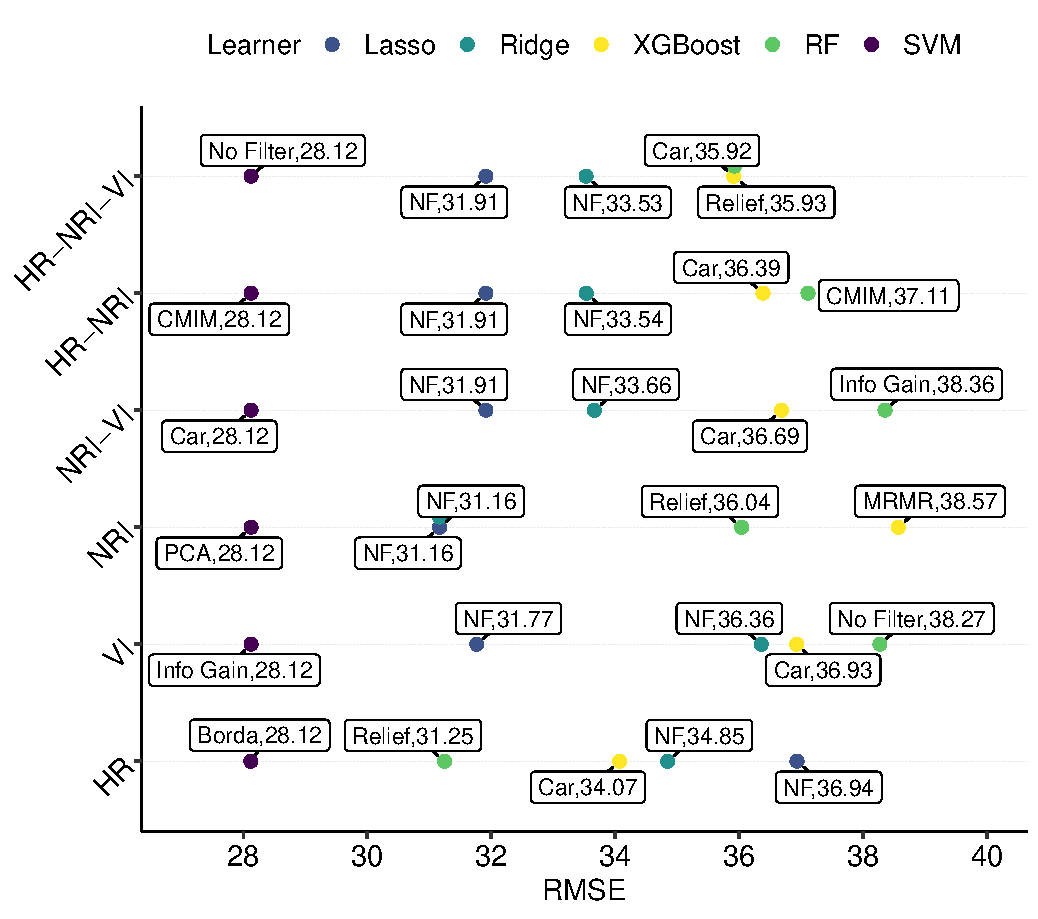
\includegraphics[width=0.48\textwidth] {performance-results-1.pdf}
		\caption{Predictive performance (RMSE) of models across tasks. Suffix 'CV' denotes that the learner was optimized using internal 10-fold CV while prefix 'MBO' means that model-based optimization was used for hyperparameter optimization. Abbreviations on the vertical axis refer to the combinations of feature sets on which each model was scored on. Labels represent the feature selection method (NF = no filter, Car = 'Carscore', Info = 'Information Gain', Borda = 'Borda'). The second value of each label shows the RMSE value of the respective setting.}\label{fig:perf-result}
	\end{center}
\end{figure}

% plot no filter vs all other filters for each model and task
\begin{figure} [t!]
	\centering
	\begin{center}
		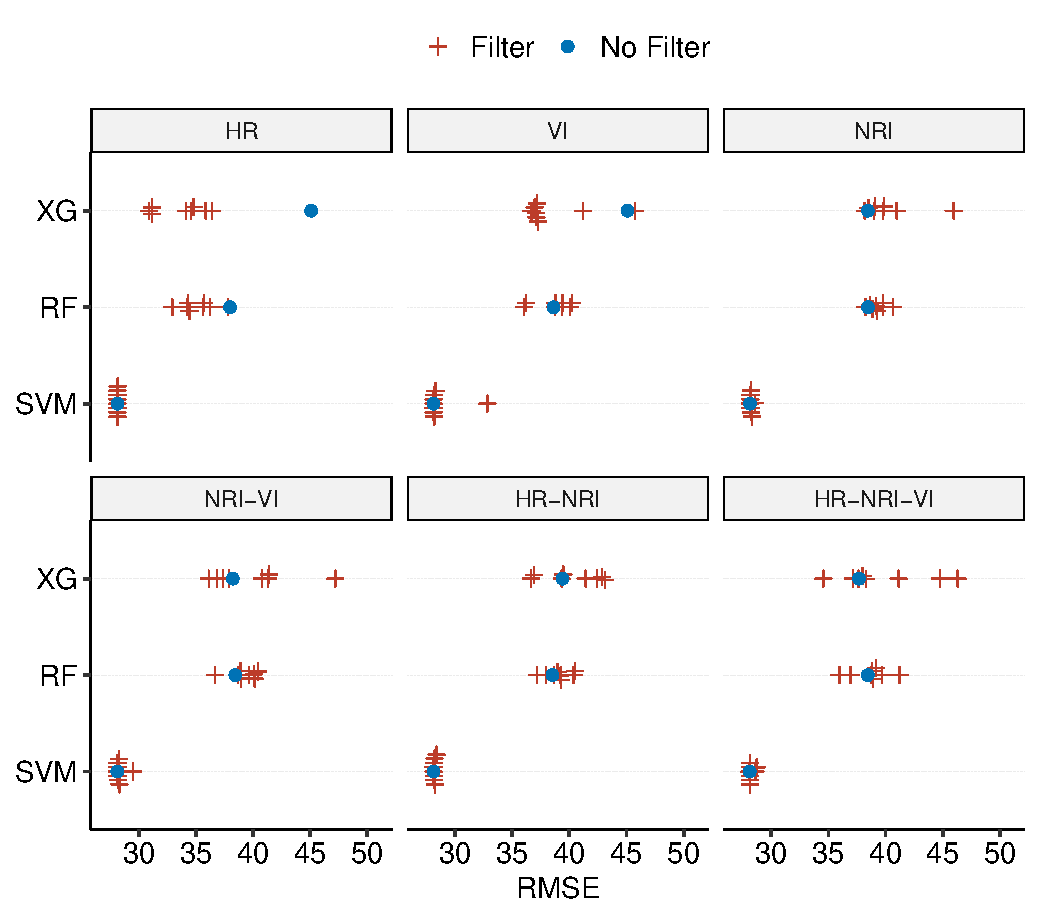
\includegraphics[width=0.48\textwidth] {filter-effect-all-vs-no-filter-1.pdf}
		\caption{Model performances in RMSE when using no filter method compared to all other filters across all tasks.}\label{fig:filter-effects-no-filter}
	\end{center}
\end{figure}

% plot Borda vs all other filters for each model and task
\begin{figure} [t!]
	\centering
	\begin{center}
		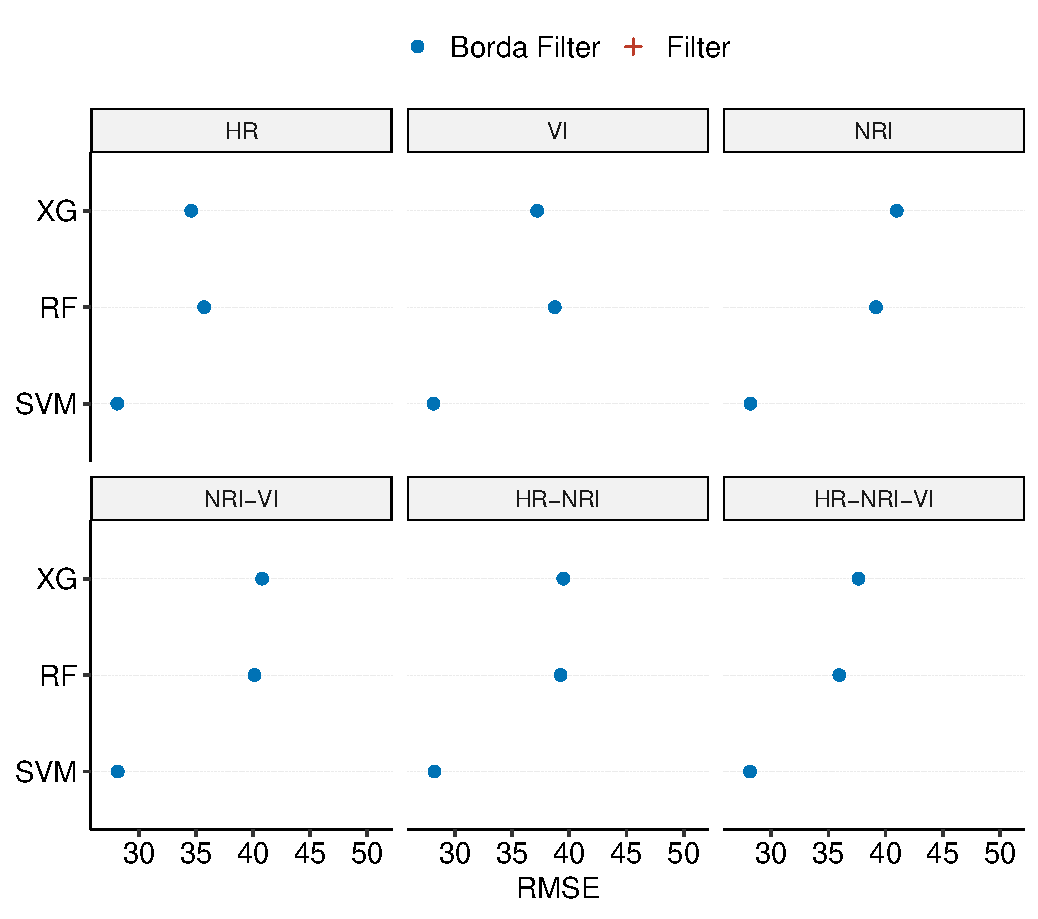
\includegraphics[width=0.48\textwidth] {filter-effect-all-vs-borda-filter-1.pdf}
		\caption{Predictive performances in RMSE when using the Borda filter method compared to all other filters for each learner across all tasks.}\label{fig:filter-effects-borda}
	\end{center}
\end{figure}

\subsection{Variable importance}

\subsubsection{Permutation-based Variable Importance}

% Variable Importance
% - VI: Vogelmann indices are best
% - All: Clustering around the red edge (700 - 750 nm)
% - Overall highest: 1.7 RMSE decrease - not that much

The most important features for datasets HR and VI showed an average decrease in RMSE of 1.57 p.p. (HR, B69) and 1.79 p.p (VI, Vogelmann2) (\autoref{fig:fi-permut-vi-hr}).
For both datasets most features among the ten most important ones cluster around a wavelength range of 700 nm - 750 nm (the so called \enquote{red edge}).
For feature set HR, four features in the infrared region (920 nm - 1000 nm) were identified by the model to be most important (causing a mean decrease in RMSE of around 1 percentage point).
Overall, most features showed only a small importance with average decreases in RMSE below 0.5 p.p..

% permutation based var imp for datasets HR and VI
\begin{figure*} [ht!]
	\centering
	\begin{center}
		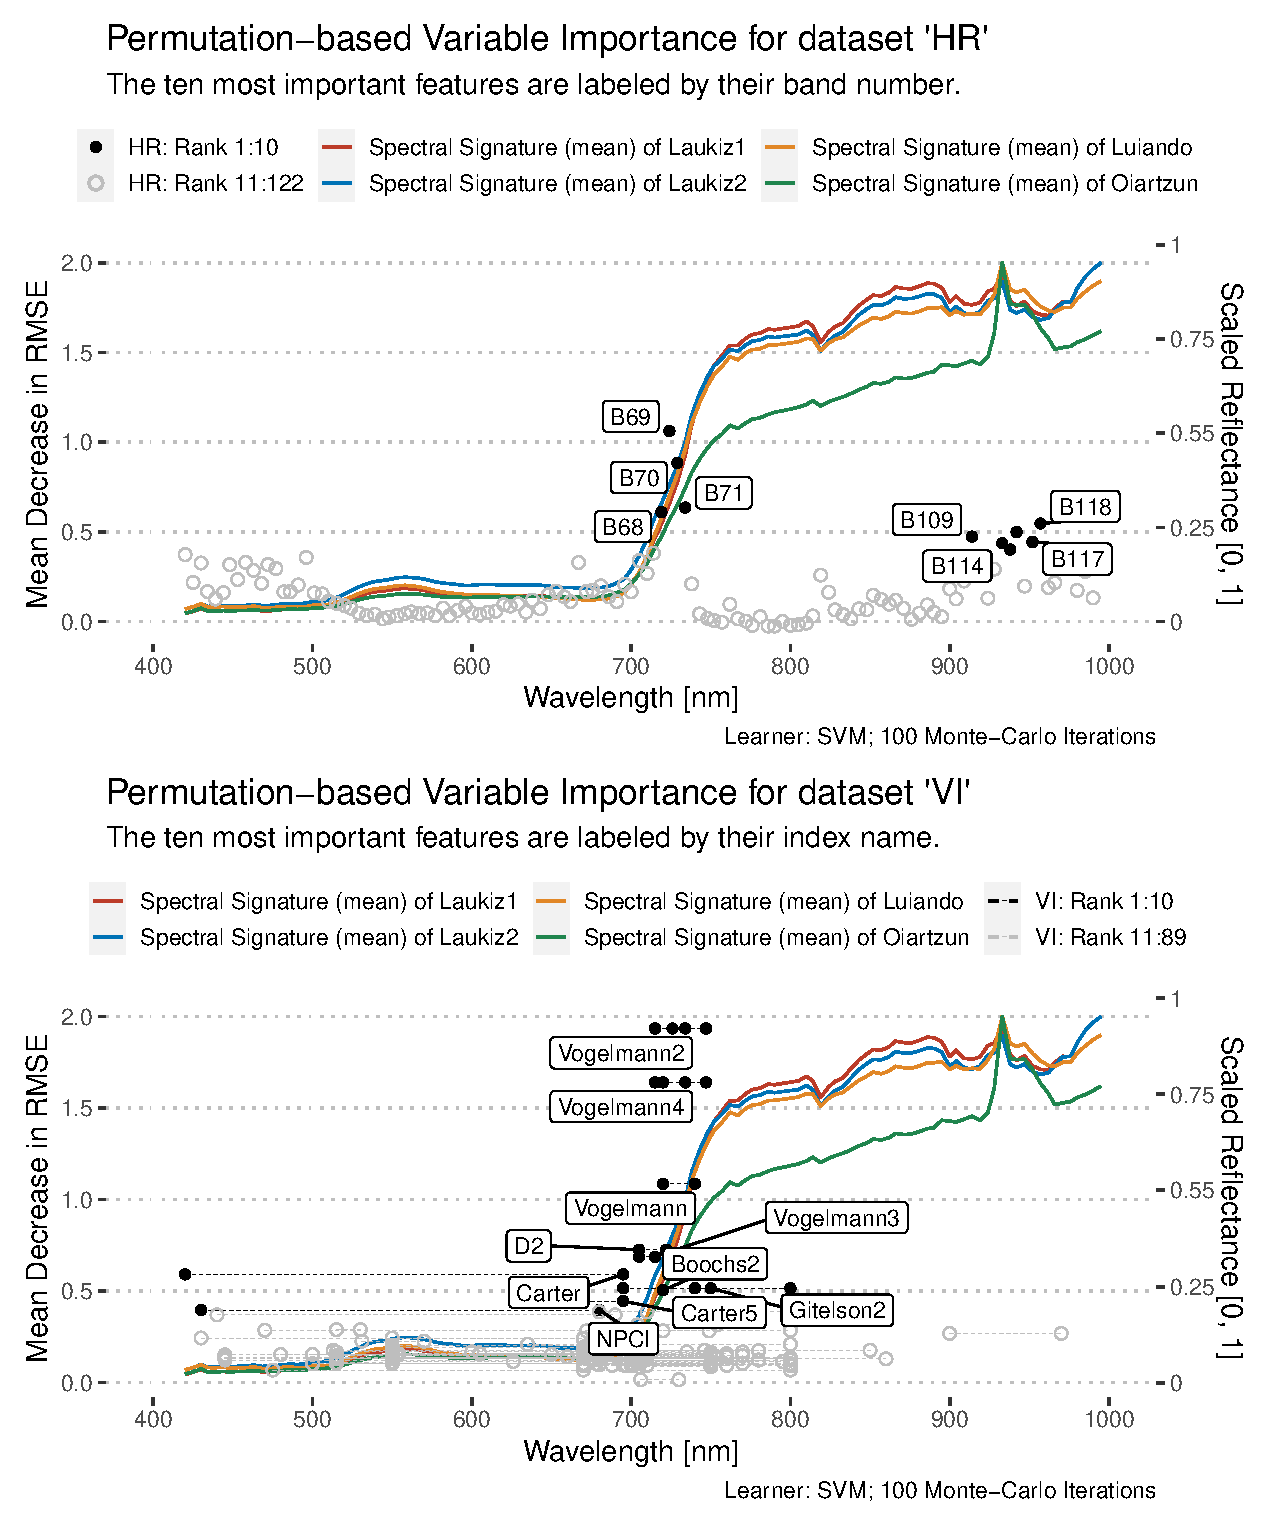
\includegraphics[width=0.9\textwidth] {fi-permut-vi-hr-1.pdf}
		\caption{Variable importance for feature sets HR and VI: Mean decrease in RMSE for one-hundred feature permutations using the SVM learner. The wavelength range on the x-axis matches the range of the hyperspectral sensor (400 nm - 1000 nm). For each dataset, the ten most important features were highlighted as black dots and labeled by name. Grey dots represent features from importance rank 11 to last. The spectral signature (mean) of each plot was added as a reference on a normalized reflectance scale [0, 1] (secondary y-axis). VI features were decomposed into their individual formula parts; all instances being connected via dashed lines. Each VI feature is composed out of at least two instances.}\label{fig:fi-permut-vi-hr}
	\end{center}
\end{figure*}

\subsubsection{ALE Plots}

Most ALE plots show a small absolute change in ALE compared to their respective mean effects (= 0) for all chosen features (less than $\pm 0.001$) (\autoref{fig:fi-hr-ale}).
Also, a medium-to-high relative dynamic over the respective reflectance value range of each variable was observed.

\section{Discussion}

\subsection{Predictive Performance}

The best aggregated performance of this study (SVM + \enquote{Info Gain} filter, RMSE 27.99 p.p.) has to be seen in the light of model overfitting (see \autoref{subsec:perf-plot-char}).
Leaving out the performance on Laukiz2 when aggregating results, the mean RMSE would be around 19 percentage points.
However, leaving out a single plot would also change the prediction results for the other plots because the observations from Laukiz2 would not be available for model training.
Due to the apparent presence of model overfitting in this study it can be postulated that more training data representing a greater variety of situations is needed.
A model can only make robust predictions if it has learned relationships across the whole range of the response.
Hence, care should be taken when predicting to the landscape scale using models fitted on this dataset due to their lack of generalizability caused by the limitations of the available training data.
However, when inspecting the fold level performances, it can be concluded that the model performed reasonably well predicting defoliation greater than 50\% but failed for lower levels.
This applied to all learners of this study.

\subsubsection{Model differences}

An interesting finding is the strength of the SVM algorithm when comparing its predictive performance to its competitors (\autoref{tab:best-learner-perf}).
These cluster around a performance of 31 p.p while SVM is able to score about 3 p.p. better than all other methods.
However, we refrain from comparing these results (both relatively and absolute) to other studies since many study design points have an influence on the final result (optimization strategy, data characteristics, feature selection methods, etc.).

Penalized methods showed promising performances, especially when taking runtime into account.
When removing features with a correlation of nearly 1, lasso is able to score performances around 31 p.p. and shows, somewhat surprisingly, the best performance on the VI task.
The same general conclusion applies to ridge if one discards the problematic results on four tasks.
Regarding the problematic predictions of the ridge learner, a careful inspection of the hyperparameter optimization procedure of the fitted models ensured again that everything was correctly implemented.
One observation turned out to be influential in causing the outlier prediction value even though careful multivariate exploratory data analysis showed no reason for flagging this observation a priori.
It was therefore left in the model, but it should be acknowledged that this learner seemed particularly sensitive to the input data.

A potential limiting factor in this study could be the upper limit of 600 iterations used for the XGBoost algorithm (hyperparameter \texttt{nrounds}), especially for feature sets including NRIs (\autoref{tab:hyperparameter_limits}).
This setting was a compromise between runtime and tuning space extension with the goal to work well for most feature sets.
It may be recommendable to increase this upper limit to a value closer to the number of features in the dataset in order to be able to exploit the full potential of this hyperparameter.

\subsubsection{Feature set differences}

One objective of this study was whether expert-based or data-driven feature engineering has a positive influence on model performance.
With respect to \autoref{fig:perf-result}, no overall positive or negative trend was found for all models that related to specific feature sets.
The performance of RF and XGBoost on the VI feature set was about six percentage points lower than on others.
One reason could be the lack of coverage in the wavelength area between 810 nm and 1000 nm (\autoref{fig:fi-permut-vi-hr}).
In addition, for all learners but SVM a better performance was observed when NRI indices were included in the feature set (i.e. NRI-VI, HR-NRI, HR-NRI-VI).

\subsection{Performance vs.\ plot characteristics}
\label{subsec:perf-plot-char}

The large differences in RMSE obtained on different test folds can be attributed to model overfitting (\autoref{tab:svm-single-fold-perf}).
An RMSE of 54.26 p.p. reveals the model's inability to predict tree defoliation on this plot (Laukiz2).
Laukiz2 differs highly in the distribution of the response variable defoliation compared to all other plots (\autoref{fig:defol-distr}).
In the prediction scenario for Laukiz2, the model was trained on data containing mostly medium-to-high defoliation values and only few low ones.
This caused overfitting on the medium-to-high values, degrading the model's predictive performance in other scenarios.
When Laukiz2 was in the training set, the overall mean RMSE was reduced by up to 50\% with single fold performances as good as 9 p.p. RMSE (with Luiando as test set).

The large differences of selected features per fold during tuning give interesting insights into internals of the used models (\autoref{tab:tune-perc-sel-features}).
While in most cases, SVM and XGBoost require a substantial portion of all available features to achieve robust predictions, RF was able to achieve the best results with a relatively small amount of features.
Realizing early that few features are needed during tuning to reach adequate performances can reduce the overall computational runtime substantially, especially when iterating over parameters such as $m_\textrm{try}$ whose optimum (and range) depends on the number of features.
Hence, regardless of the potential advantage of using filters for increased predictive performance, it should be noted that these can have a strong positive effect on runtime, at least for RF in this study.

Ultimately, the results of \autoref{tab:tune-perc-sel-features} should be taken with care as they rely on single model-filter combinations and are subject to random variation.
More in-depth research is needed to investigate the effect of filters on other criteria than performance (such as runtime), leading to a multi-criteria optimization problem.

\subsection{Feature selection methods}

% - Effect varies across learners -> suggest to use FS even on feature sets with p < 100?
% - Filters can also have a negative impact
% - Filters are interesting for reducing runtime and improve interpretability, not only for performance
The usefulness of filters with respect to predictive performance in this study varied.
While the performance of some models (up to 5 p.p. for RF and XGBoost) was improved by specific filters, some models achieved a poorer performance with filters than without them (\autoref{fig:filter-effects-no-filter}).
Since these negative cases were not caused by a specific filter method, it is recommended to test multiple filters in a study if filters are going to be used.
While filters can improve the performance of models, they might be more interesting in other aspects than performance: reducing variables can reduce computational efforts in high-dimensional scenarios and might enhance the interpretability of models.
Filters are a lot cheaper to compute than wrapper methods and the final feature subset selection can be added as an additional hyperparameter to the model optimization stage.

% - Ensemble FS shows no advantage to simple methods -> always one simple filter which is better. Ensemble filters are good across many different datasets
The models which used the Borda ensemble method in this study did not score better on average than models which used a single filter or no filter at all.
Ensemble methods have higher stability and robustness than single ones and have shown promising results in \cite{drotar2017a}.
Hence, their main advantage are stable performances across datasets with varying characteristics.
Single filter methods might yield better model performances on certain datasets but fail on others.
The fact that this study used multiple feature sets but only one dataset and tested many single filters could be a potential explanation why in almost all cases (besides XGBoost on task HR-NRI-VI) a single filter outperformed the ensemble filter.
However, studies which used ensemble filters are still rare and usually these are not compared against single filters \cite{ghosh2019}.
In summary, Borda performs no better than a randomly selected filter method in this study.
More case studies applying ensemble filter methods are needed to verify this finding.
Nevertheless, ensemble filters can be a promising addition to a machine-learning feature-selection portfolio.

% - PCA shows similar performance but probably requires tuning of main components -> check runtime!
PCA, acting as a filter method in this work, did neither show the best nor worst result compared to other feature-selection approaches.
It was able to reduce model fitting times substantially.
Depending on the use case, PCA can be an interesting option to reduce dimensionality while keeping runtime low.
However, information about the total number of features used by the model is lost when applying this technique.
Since filter scores only need to be calculated once for a given dataset in a benchmark setting, the runtime advantage of a PCA vs. filter methods might in fact be negligible in practice.

\subsection{Linking feature importance to spectral characteristics}

Not surprisingly the most important features for both HR and VI datasets were identified around the red edge of the spectra, specifically in the range of 680 nm to 750 nm.

This area has the highest ability to distinguish between reflectances related to a high density / high foliage density und thus the health status of vegetation and its respective counterpart \cite{horler1983}.
However, four out of ten of the most important features of dataset HR are located between 920 nm and 1000 nm.
Looking at the spectral curves of the plots, apparent reflectance differences can be observed in this spectral area - especially for plot Oiartzun - which might explain why these features were considered important by the model.

A possible explanation for the worse performances of most models scored on the VI dataset compared to all other feature sets could be the lack of features covering the area between 850 nm and 1000 nm (\autoref{fig:fi-permut-vi-hr}).
The majority of VI features covers the range between 550 nm - 800 nm.
Only one index (PWI) covers information in the range beyond 900 nm.

% ALE plots
The ALE plots are hard to interpret because their values are interpreted on a relative scale and differ for each band.
When linking band reflectance values against ALE values of a specific band, a value of 100 has a very different meaning in B67 than in B124 because for the latter, reflectance values of vegetation are naturally higher.
Hence, a reflectance value of 100 would be considered high for B67 but low for B124 with respect to a spectral curve of vegetation.
However, no baseline reflectance value for every feature exists since the absolute reflectance values depend on the sensor characteristics.
ALE plots can be a powerful tool for interpreting feature importance of correlated features but might be limited in their interpretability because only relative comparisons can be conducted.

\subsection{Data quality}

Environmental datasets always come with some constraints that can have potential influence on the modeling process and its outcome.
The following paragraph discusses these.
The decision to use a buffer of two meters for the extraction of reflectance values was a complex process.
Due to the reported geometric offset of up to 1 m within the hyperspectral data, the risk of assigning a value to an observation which would actually refer to a different observation was reasonably high.
By using a buffer of two meters (or more), the probability of including information from other trees into the final value increases, blurring the actual value of the tree observation.
However, when using no buffer at all, the difference between single, neighboring pixels might even be higher compared to a smoothed value composed out of a buffer.
It was concluded that using a buffer of two meters is a good compromise between the inclusion of information from too many surrounding trees and not accounting for the geometric offset at all.
Even though no results showing the influence of multiple buffer values on the extraction were provided, it is hypothesized that the relationships between features would not change substantially, leading to almost identical model results.

Another point worth discussing is that the exact number of contributing pixels to the final index value of an observation cannot be determined precisely: it depends on the location of the tree within the pixel grid.
According to the extract function of the raster package, a pixel is included if its centroid (and not just any part of the grid cell) falls inside the buffer.
As the buffer is circular, the total number of contributing pixels of each tree depends on the exact location of a tree within the pixel grid.
If a tree observation is located on the border of the plot, some directions of the buffer will contain no values and the subsequent index value will be calculated with fewer pixels than if the tree observation is located in the middle of the plot.

The available hyperspectral data covered a wavelength between 400 nm and 1000 nm.
Hence, the wavelength range of the shortwave infrared (SWIR) region is not covered in this study.
Given that this wavelength range is often used in forest health studies \cite{hais2019}, e.g. when calculating the \ac{NDMI} index \cite{gao1996}, this marks a clear limitation of the dataset at hand.

The R package hsdar was used for the calculation of vegetation indices \cite{lehnert2016}.
All indices that could be calculated with the given spectral range of the data (400 nm - 1000 nm) were used.
This means even though \autoref{tab:vegindices} lists all available indices of the package, not all listed indices were used in this study.
Even though this selection included a large number of indices, some possibly helpful indices might have been missed due to the restriction of the hyperspectral data.

Overall, the magnitude of uncertainty introduced by the mentioned effects during index derivation cannot be quantified.
Such limitations and uncertainties apply to most environmental studies and cannot be completely avoided.

\subsection{Comparison to other studies}
% - no environmental studies use filter methods, some use FFS
% - only few studies analyze defoliation
% - most FS is done in bioinformatics

While most defoliation studies operate on the plot level using coarser-resolution multispectral satellite data \cite{townsend2012, debeurs2008, rengarajan2016}, there are also several recent studies using airborne or ground-based sensors at the tree level.
Among these, \cite{meng2018, kalin2019} used ground-level methods such as \ac{ALS} or \ac{LiDAR}.

Studies focusing on tree-level defoliation used ground-level methods such as \ac{ALS} or \ac{LiDAR}\cite{meng2018, kalin2019}.
\cite{meng2018} used \ac{OLS} regression methods while \cite{kalin2019} retrieved information from ground-level RGB photos using \ac{CNN}.
However, both did not use spatial \ac{CV} and \cite{kalin2019} no \ac{FS}.
\cite{goodbody2018} used a \ac{PLS} model with high-resolution \ac{DAP} to predict cumulative defoliation caused by the spruce budworm.
Study results indicated that spectral features were found to be most helpful for the model.
Incorporating such (both spectral and structural) could be a possible enhancement for future works.

% write about hyperspectral remote sensing
The field of (hyperspectral) remote sensing has a strong focus on using random forests for modeling in recent years \cite{belgiu2016}.
However, in high-dimensional scenarios, tuning parameter \texttt{\(m_{try}\)} becomes computationally expensive.
To account for this and the high dimensionality in general, studies used feature selection approaches like semi-supervised feature extraction \cite{xia2015}, wrapper methods \cite{fassnacht2014, feng2016, georganos2018}, PCA and adjusted feature selection \cite{rochac2016}.
However, no study that made use of filter methods in combination with hyperparameter tuning in the field of (hyperspectral) remote sensing could be found.
Potential reasons for this gap could be an easier access to wrapper methods and a higher general awareness of such compared to filter methods.
Applying the filter-based feature selection methodology shown in this study and its related code provided in the research compendium might be a helpful reference for future studies using hyperspectral remote sensing data.

% RS studies with more/other algorithms than RF
When looking for remote sensing studies that compare multiple models, it turned out that these often operate in a low-dimensional predictor space \cite{xu2019} or use wrapper methods explicitly \cite{georganos2018}.

\cite{shendryk2016, ludwig2019} are more similar in their methodology but focus on a different response variable (woody cover).
\cite{shendryk2016} used machine learning with \ac{ALS} data to study dieback of trees for eucalyptus forests.
A grid search was used for hyperparameter tuning and \ac{FFS} for variable selection.
\cite{ludwig2019} analyzed woody cover in South Africa using spatial \ac{CV} and \ac{FS} approach \cite{meyer2018} with a random forest classifier.
\cite{zandler2015} shows a similar setup: they used hyperspectral vegetation indices, a nested CV approach for performance estimation and estimated variable importance targeting woody biomass as the response.
In the results, lasso showed the best performance among the chosen methods.
However, the authors did not optimize the hyperparameters of RF which makes a fair comparison problematic since the other models used perform internal optimization.
The discussion section of \cite{zandler2015} lists additional studies that made use of shrinkage models for high dimensional remote sensing modeling.

In summary, no studies which used filter methods for \ac{FS} or made use of \ac{NRI} indices in their work and had a relation to tree health were found.
This might relate to the fact that most environmental datasets are not high-dimensional.
In fact, many studies use fewer than ten features and issues related to correlations are often solved manually instead of relying on an automated approach.
This can be subjective and may limit the reproducibility of results.

Other fields (e.g. bioinformatics) face high-dimensional datasets more often.
Hence more studies using (filter-based) feature-selection approaches can be found for this field \cite{guo2019, radovic2017}.
Yet bioinformatics differs conceptually in many ways from environmental modeling and therefore no greater focus was put into comparing studies of this field.
The availability of high dimensional feature sets will increase in the future due to higher temporal and spectral resolutions of sensors.
In addition, a high spatial resolution comes with the possibility to calculate many textural features.
Hence, the ability to deal with high dimensional datasets becomes more important and unbiased robust approaches are needed.
We hope that this work and its methodology raises awareness about the application of filter methods to tackle high-dimensional problems in the environmental modeling field.

\section{Conclusion}

This study analyzed defoliation of trees in northern Spain by using hyperspectral data as input for machine-learning models which used hyperparameter tuning and filter-based feature selection.
Substantial differences in performance occurred depending on which feature selection and machine learning methods were combined.
SVM showed the most robust behavior across all highly-correlated datasets and was able to predict the response variable of this study substantially better than other methods.

% RQ3: How are feature-selection methods influencing the predictive performance of the models?
Filter methods were able to improve the predictive performance on datasets in some instances, although there was no clear and systematic pattern.
Their effectiveness depends on the algorithm and the dataset characteristics.
Ensemble filter methods did not show a substantial improvement over individual filter methods in this study.

% RQ2: Does combining feature sets have an substantial effect on predictive performance?
% RQ1: Do different environmental feature sets show differences in performance when modeling defoliation at trees?
The addition of derived feature sets was in most cases able to improve predictive performance.
In contrast, feature sets which focused on only a small fraction of the available spectral range (i.e. dataset VI) showed a worse performance than the ones which covered wider range (400 nm - 1000 nm; HR, NRI).
NRIs can be seen as a valuable addition for optimizing predictive performance in remote sensing of vegetation.

% RQ4: Which features are most important for the models and how can these be interpreted in an ecological context?
Features along the red edge wavelength region were most important for models during prediction.
With respect to dedicated vegetation indices, all versions of the Vogelmann index were seen as the most important index for the best performing SVM model.
This matches well with the actual purpose of these indices:
These were invented to detect defoliation on sugar maple trees (\textit{Acer saccharum Marsh.}) caused by pear thrips (\textit{Taeniothrips inconsequens Uzel}) \cite{vogelmann1993}.
However, assessing the feature importance for highly correlated features remains a challenging task.
Results might be biased and should be taken with care to avoid overgeneralizing from individual studies.

% What about the general potential of analyzing defol with hyperspectral data?
Finally, the potential of predicting defoliation with the given study design was rather limited with respect to the average RMSE of 27 percentage points scored by the best performing model.
More training data covering a wider range of defoliation values in a larger number of forest plantations is needed to train better models which can create more robust predictions.

\section{Acknowledgments}
This work was funded by the EU LIFE Healthy Forest project (LIFE14 ENV/ES/000179) and the German Scholars Organization/Carl Zeiss Foundation.

\appendices{}

\section{SVM ALE plots for task HR}

\begin{figure} [ht]
	\begin{center}
		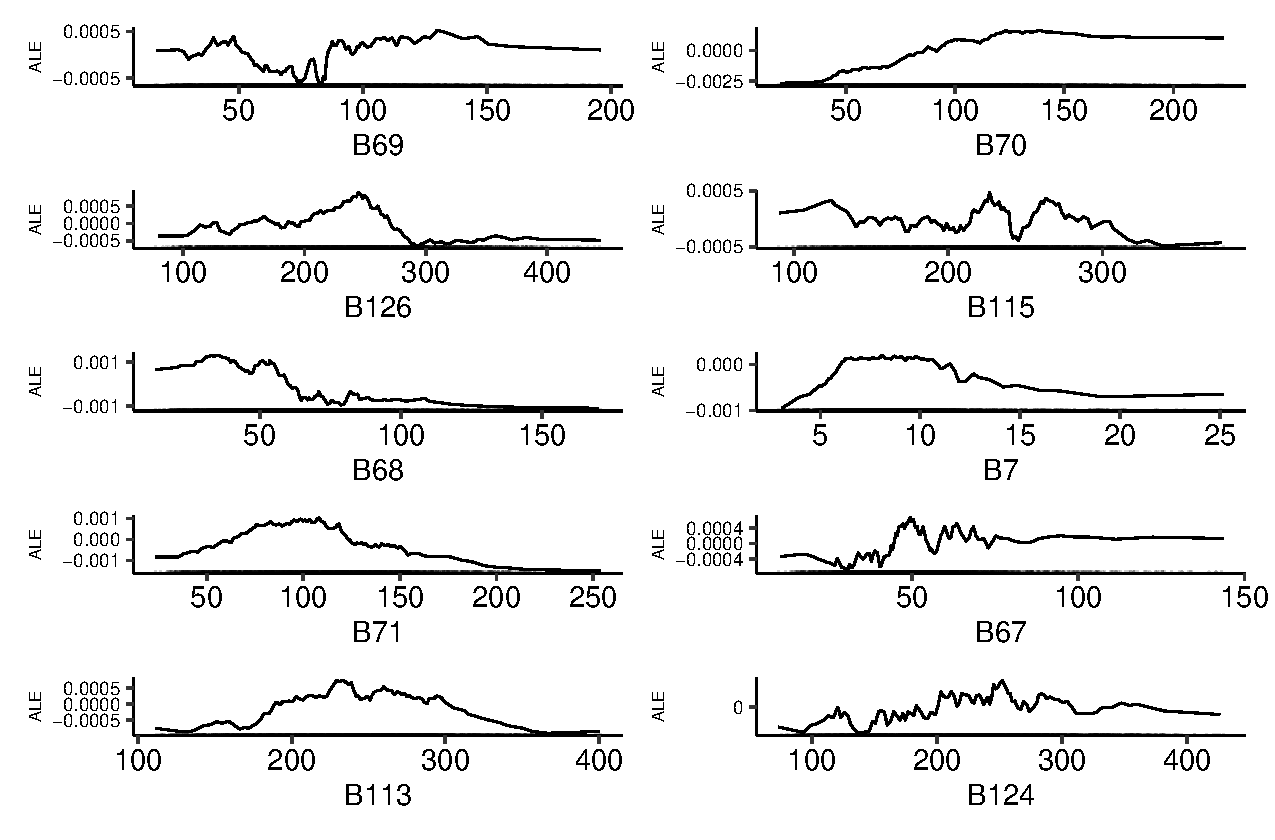
\includegraphics[width=0.48\textwidth] {fi-hr-ale-1.pdf}
		\caption{ALE plots of SVM on dataset HR. The ten most important features from the permutation-based variable importance estimation were used. The y-axis shows the deviation to the mean prediction for each feature, with the mean prediction being centered at zero.}\label{fig:fi-hr-ale}
	\end{center}
\end{figure}

%\section{SVM ALE plots for task VI}

% \begin{figure} [ht]
% 	\begin{center}
% 		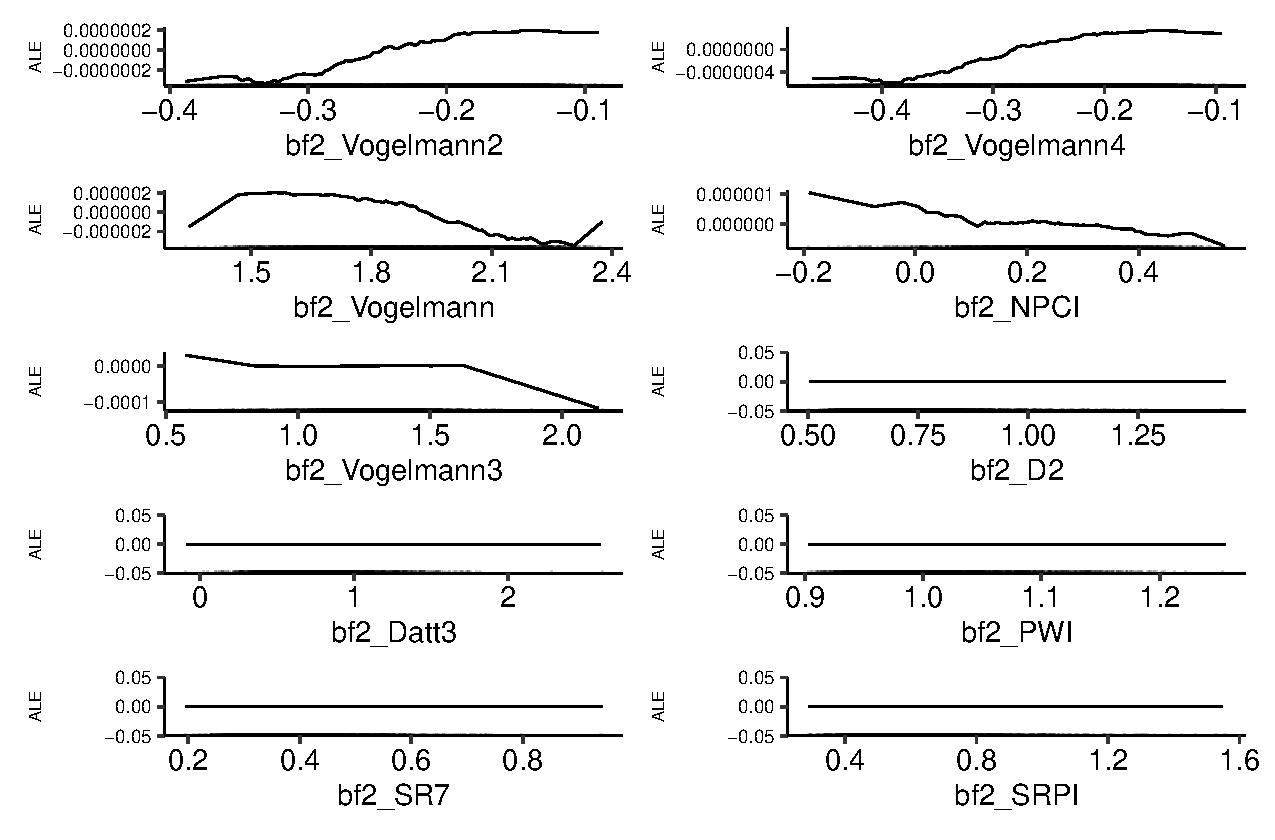
\includegraphics[width=0.48\textwidth] {fi-vi-ale-1.pdf}
% 		\caption{ALE plots on dataset VI of SVM learner. Subset showing the ten most important features according to the permutation-based variable importance. The y-axis shows the deviation to the mean prediction for each feature, with the mean prediction being centered at zero.}\label{fig:fi-vi-ale}
% 	\end{center}
% \end{figure}

\pagebreak
\section{Correlation among filter methods}

\begin{figure} [ht]
	\begin{center}
		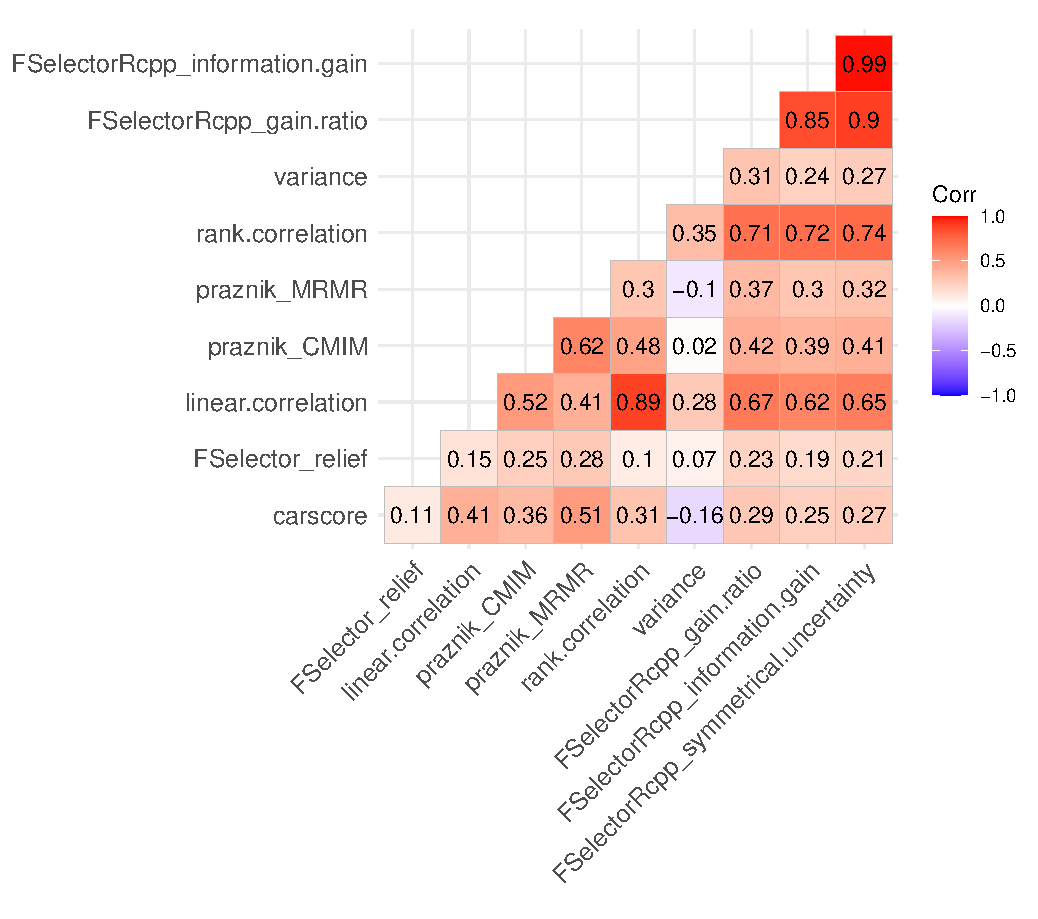
\includegraphics[width=0.48\textwidth] {correlation-filter-nri-1.pdf}
		\caption{Spearman correlations of NRI feature rankings obtained with different filters.}\label{fig:correlation-filters}
	\end{center}
\end{figure}

\section{Effect of different \texorpdfstring{\(n_{bins}\)}{nbins} values on filter 'information gain'}

\begin{figure} [ht]
	\begin{center}
		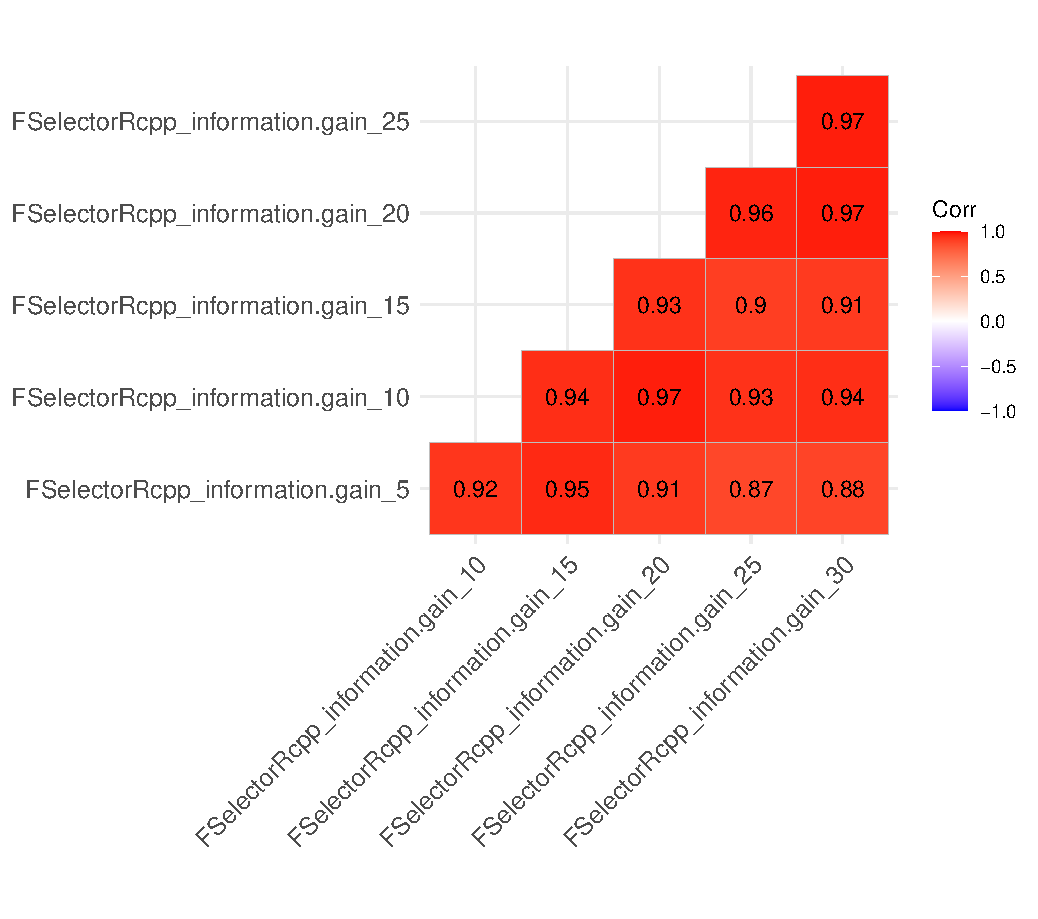
\includegraphics[width=0.48\textwidth] {correlation-nbins-1.pdf}
		\caption{Spearman correlations of rankings obtained with the information gain filter using different \texttt{\(n_{bins}\)} values for discretization of the numeric response.}\label{fig:correlation-nbins}
	\end{center}
\end{figure}

\pagebreak

\section{Hyperparameter tuning ranges}

% parameter limits
\begin{table}[b!]
	\centering
	\caption[t]{Hyperparameter ranges and types for each model.
		Hyperparameter notations from the respective R packages were used.}
	\begingroup\scriptsize
	\begin{tabularx}{.5\textwidth}{llXXrXX}
		\\
		\specialcell{Model                                              \\ (package)}                & Hyperparameter              & Type    & Start     & End      & Default \\
		\toprule
		\multirow{3}{*}{\specialcell{RF                                 \\ (ranger)}}       & \texttt{$x_try$}    & dbl & 0         & 0.5      & -       \\
		 & \texttt{min.node.size}      & int & 1        & 10      & 1   \\
		 & \texttt{sample.fraction}    & dbl & 0.2      & 0.9     & 1   \\
		\midrule
		\multirow{2}{*}{\specialcell{SVM                                \\ (kernlab)}}     & \texttt{C}                  & dbl & $2^{-10}$ & $2^{10}$ & 1       \\
		 & \texttt{$\sigma$}           & dbl & $2^{-5}$ & $2^{5}$ & 1   \\
		\midrule
		\multirow{7}{*}{\specialcell{XGBoost                            \\ (xgboost)}} & \texttt{nrounds}            & int & 10        & 600      & -       \\
		 & \texttt{colsample\_bytree}  & dbl & 0.3      & 0.7     & 1   \\
		 & \texttt{subsample}          & dbl & 0.25     & 1       & 1   \\
		 & \texttt{max\_depth}         & int & 1        & 10      & 6   \\
		 & \texttt{gamma}              & int & 0        & 10      & 0   \\
		 & \texttt{eta}                & dbl & 0.01     & 0.6     & 0.3 \\
		 & \texttt{min\_child\_weight} & int & 0        & 20      & 1   \\
		\bottomrule
	\end{tabularx}
	\endgroup
	\label{tab:hyperparameter_limits}
\end{table}

\begingroup\scriptsize
\setlength\tabcolsep{4pt}  % default value: 6pt
\begin{xtabular*}{0.3\textwidth}{lll}
	\bfseries{Name} & \bfseries{Formula}                                                                                  & \bfseries{Reference*}      \\
	Boochs          & $D_{703}$                                                                                           & \cite{boochs1990}       \\
	Boochs2         & $D_{720}$                                                                                           & \cite{boochs1990}       \\
	CAI             & $0.5 \times (R_{2000} + R_{2200}) -R_{2100}$                                                        & \cite{nagler2003}       \\
	\midrule
	CARI            & $a = (R_{700}-R_{550}) / 150$                                                                       & \cite{walthall1994}          \\
	& $b = R_{550}-(a\times 550)$                                                                                         &                                  \\
	& $\frac{R_{700}\times | (a\times 670+R_{670}+b)}{R_{670}\times(a^2+1)| ^{0.5}}$                                      &                                  \\
	\midrule
	Carter          & $R_{695}/R_{420}$                                                                                   & \cite{carter1994}              \\
	Carter2         & $R_{695}/R_{760}$                                                                                   & \cite{carter1994}              \\
	Carter3         & $R_{605}/R_{760}$                                                                                   & \cite{carter1994}              \\
	Carter4         & $R_{710}/R_{760}$                                                                                   & \cite{carter1994}              \\
	Carter5         & $R_{695}/R_{670}$                                                                                   & \cite{carter1994}              \\
	Carter6         & $R_{550}$                                                                                           & \cite{carter1994}              \\
	CI              & $R_{675}\times R_{690}/R_{683}^2$                                                                   & \cite{zarco-tejada2003a} \\
	CI2             & $R_{760}/R_{700}-1$                                                                                 & \cite{gitelson2003}     \\
	ClAInt          & $\int_{600 nm}^{735 nm} R$                                                                          & \cite{oppelt2004}   \\
	CRI1            & $1/R_{515}-1/R_{550}$                                                                               & \cite{gitelson2003}     \\
	CRI2            & $1/R_{515}-1/R_{770}$                                                                               & \cite{gitelson2003}     \\
	CRI3            & $1/R_{515}-1/R_{550}\times R_{770}$                                                                 & \cite{gitelson2003}     \\
	CRI4            & $1/R_{515}-1/R_{700}\times R_{770}$                                                                 & \cite{gitelson2003}     \\
	D1              & $D_{730}/D_{706}$                                                                                   & \cite{zarco-tejada2003a} \\
	D2              & $D_{705}/D_{722}$                                                                                   & \cite{zarco-tejada2003a} \\
	Datt            & $(R_{850}-R_{710})/(R_{850}-R_{680})$                                                               & \cite{datt1999}               \\
	Datt2           & $R_{850}/R_{710}$                                                                                   & \cite{datt1999}               \\
	Datt3           & $D_{754}/D_{704}$                                                                                   & \cite{datt1999}               \\
	Datt4           & $R_{672}/(R_{550} \times R_{708})$                                                                  & \cite{datt1998}                \\
	Datt5           & $R_{672}/R_{550}$                                                                                   & \cite{datt1998}                \\
	Datt6           & $(R_{860})/(R_{550}\times R_{708})$                                                                 & \cite{datt1998}                \\
	Datt7           & $(R_{860} - R_{2218})/(R_{860} - R_{1928})$                                                         & \cite{datt1999a}               \\
	Datt8           & $(R_{860} - R_{1788})/(R_{860} - R_{1928})$                                                         & \cite{datt1999a}               \\
	DD              & $(R_{749}-R_{720})-(R_{701}-R_{672})$                                                               & \cite{maire2004}     \\
	DDn             & $2\times (R_{710}-R_{660}-R_{760})$                                                                 & \cite{lemaire2008}     \\
	DPI             & $(D_{688}*D_{710})/D_{697}^2$                                                                       & \cite{zarco-tejada2003a} \\
	DWSI1           & $R_{80}/R_{1660}$                                                                                   & \cite{apan2004}         \\
	DWSI2           & $R_{1660}/R_{550}$                                                                                  & \cite{apan2004}         \\
	DWSI3           & $R_{1660}/R_{680}$                                                                                  & \cite{apan2004}         \\
	DWSI4           & $R_{550}/R_{680}$                                                                                   & \cite{apan2004}         \\
	DWSI5           & $(R_{800} + R_{550})/(R_{1660} + R_{680})$                                                          & \cite{apan2004}         \\
	EGFN            & $\frac{(\max(D_{650:750})-\max(D_{500:550}))}{(\max(D_{650:750})+\max(D_{500:550}))}$               & \cite{penuelas1994}     \\
	EGFR            & $\max(D_{650:750})/\max(D_{500:550})$                                                               & \cite{penuelas1994}     \\
	EVI             & $\frac{2.5\times ((R_{800}-R_{670}) }{ (R_{800}-(6\times R_{670})-(7.5\times R_{475})+1)}$          & \cite{huete1997a}        \\
	GDVI            & $(R_{800}^n-R_{680}^n) / (R_{800}^n+R_{680}^n)$**                                                   & \cite{wu2014}                  \\
	GI              & $R_{554}/R_{677}$                                                                                   & \cite{smith1995}        \\
	Gitelson        & $1/R_{700}$                                                                                         & \cite{gitelson1999}     \\
	Gitelson2       & $(R_{750}-R_{800}/R_{695}-R_{740})-1$                                                               & \cite{gitelson2003}   \\
	GMI1            & $R_{750}/R_{550}$                                                                                   & \cite{gitelson2003}     \\
	GMI2            & $R_{750}/R_{700}$                                                                                   & \cite{gitelson2003}     \\
	Green NDVI      & $\frac{R_{800}-R_{550}}{R_{800}+R_{550}}$                                                           & \cite{gitelson1996}     \\
	LWVI\_1         & $\frac{(R_{1094}-R_{983})}{(R_{1094}+R_{983})}$                                                     & \cite{galvao2005}       \\
	LWVI\_2         & $\frac{R_{1094}-R_{1205}}{R_{1094}+R_{1205}}$                                                       & \cite{galvao2005}       \\
	Maccioni        & $\frac{R_{780}-R_{710})}{R_{780}-R_{680}}$                                                          & \cite{maccioni2001}     \\
	\midrule
	MCARI           & \parbox{5.5cm}{$((R_{700}-R_{670})-0.2\times (R_{700}-R_{550})) \times (R_{700}/R_{670})$}          & \cite{daughtry2000}     \\
	\midrule
	MCARI2          & \parbox{5.5cm}{$((R_{750}-R_{705})-0.2 \times (R_{750}-R_{550})) \times (R_{750}/R_{705})$}         & \cite{wu2008a}           \\
	\midrule
	mND705          & $\frac{(R_{750}-R_{705})}{R_{750}+R_{705}-2\times R_{445}}$ & \cite{sims2002a} \\
	mNDVI           &  $\frac{(R_{800}-R_{680})}{R_{800}+R_{680}-2 \times R_{445}}$ & \cite{sims2002a} \\
	MPRI            & $\frac{R_{515}-R_{530}}{R_{515}+R_{530}}$                                                           & \cite{hernandez-clemente2011}\\
	MSAVI           & \parbox{5.5cm}{$0.5 \times ((2\times R_{800}+1)^2-8\times (R_{800}-R_{670}))^{0.5}$}                & \cite{qi1994}\\
	MSI             & $\frac{R_{1600}}{R_{817}}$                                                                          & \cite{huntjr1989}\\
	mSR             & $\frac{R_{800}-R_{445}}{R_{680}-R_{445}}$                                                           & \cite{sims2002a} \\
	mSR2            & $\frac{(R_{750}/R_{705})-1}{R_{750}/R_{705}+1)^{0.5}}$                                              & \cite{chen1996}\\
	mSR705          & $\frac{R_{750}-R_{445}}{R_{705}-R_{445}}$                                                           & \cite{sims2002a} \\
	MTCI            & $\frac{R_{754}-R_{709}}{R_{709}-R_{681}}$                                                           & \cite{dash2007}\\
	\midrule
	MTVI            & \parbox{3.8cm}{$1.2 \times (1.2 \times (R_{800}-R_{550})-2.5 \times (R_{670}-R_{550}))$}            & \cite{haboudane2002}\\
	\midrule
	NDLI           & $\frac{log(1/R_{1754}) - log(1/R_{1680})}{log(1/R_{1754}) + log(1/R_{1680})}$                        & \cite{serrano2002} \\
	NDNI           & $\frac{log(1/R_{1510}) - log(1/R_{1680})}{log(1/R_{1510}) + log(1/R_{1680})}$                        & \cite{serrano2002} \\
	NDVI           & $\frac{R_{800}-R_{680}}{R_{800}+R_{680}}$                                                            & \cite{tucker1979} \\
	NDVI2          & $\frac{R_{750}-R_{705}}{R_{750}+R_{705}}$                                                            & \cite{gitelson1994} \\
	NDVI3          & $\frac{R_{682}-R_{553}}{R_{682}+R_{553}}$                                                            & \cite{guanter2005} \\
	NDWI           & $\frac{R_{860}-R_{1240}}{R_{860}+R_{1240}}$                                                          & \cite{gao1996} \\
	NPCI           & $\frac{R_{680}-R_{430}}{R_{680}+R_{430}}$                                                            & \cite{penuelas1994} \\
	OSAVI          & $\frac{(1+0.16) \times (R_{800}-R_{670})}{R_{800}+R_{670}+0.16 }$                                    & \cite{rondeaux1996} \\
	OSAVI2         & $\frac{(1+0.16)\times (R_{750}-R_{705})}{R_{750}+R_{705}+0.16) }$                                    & \cite{wu2008a} \\
	PARS           & $\frac{R_{746}}{R_{513}}$                                                                            & \cite{chappelle1992} \\
	PRI            & $\frac{R_{531}-R_{570}}{R_{531}+R_{570}}$                                                            & \cite{gamon1992}\\
	PRI\_norm      & $\frac{PRI \times (-1) }{RDVI\times R_{700}/R_{670}}$                                                & \cite{zarco-tejada2013a}\\
	PRI*CI2        & $PRI*CI2$                                                                                            & \cite{garrity2011} \\
	PSRI           & $\frac{R_{678}-R_{500}}{R_{750}}$                                                                    & \cite{merzlyak1999} \\
	PSSR           & $\frac{R_{800}}{R_{635}}$                                                                            & \cite{blackburn1998} \\
	PSND           & $\frac{R_{800}-R_{470}}{R_{800}-R_{470})}$                                                           & \cite{blackburn1998} \\
	PWI            & $\frac{R_{900}}{R_{970}}$                                                                            & \cite{penuelas1997} \\
	RDVI           & $\frac{R_{800}-R_{670}}{ \sqrt{R_{800}+R_{670}}}$                                                    & \cite{roujean1995} \\
	\midrule
	REP\_LE        & \parbox{3.8cm}{Red-edge position through linear extrapolation}                                       & \cite{cho2006} \\
	\midrule
	REP\_Li        & $R_{re}=\frac{R_{670}+R_{780})}{2}$                                                                  & \cite{guyot1988} \\
	& $\frac{700 + 40 \times ((R_{re} -R_{700})}{(R_{740}-R_{700}))}$ & \\
	\midrule
	SAVI           & $\frac{(1+L)\times (R_{800}-R_{670})}{(R_{800}+R_{670}+L)}$                                          & \cite{huete1988} \\
	SIPI           & $\frac{R_{800}-R_{445}}{R_{800}-R_{680}}$                                                            & \cite{pen-uelas1995} \\
	\midrule
	SPVI           & \parbox{3.8cm}{$0.4 \times 3.7 \times (R_{800}-R_{670})-1.2 \times ((R_{530}-R_{670})^2)^{0.5}$}     & \cite{vincini2006} \\
	\midrule
	SR             & $\frac{R_{800}}{R_{680}}$                                                                            & \cite{jordan1969} \\
	SR1            & $\frac{R_{750}}{R_{700}}$                                                                            & \cite{gitelson1997}\\
	SR2            & $\frac{R_{752}}{R_{690}}$                                                                            & \cite{gitelson1997}\\
	SR3            & $\frac{R_{750}}{R_{550}}$                                                                            & \cite{gitelson1997}\\
	SR4            & $\frac{R_{700}}{R_{670}}$                                                                            & \cite{mcmurtrey1994} \\
	SR5            & $\frac{R_{675}}{R_{700}}$                                                                            & \cite{chappelle1992} \\
	SR6            & $\frac{R_{750}}{R_{710}}$                                                                            & \cite{zarco-tejada1999} \\
	SR7            & $\frac{R_{440}}{R_{690}}$                                                                            & \cite{lichtenthaler1996} \\
	SR8            & $\frac{R_{515}}{R_{550}}$                                                                            & \cite{hernandez-clemente2012}\\
	SRPI           & $\frac{R_{430}}{R_{680}}$                                                                            & \cite{pen-uelas1995}\\
	SRWI           & $\frac{R_{850}}{R_{1240}}$                                                                           & \cite{zarco-tejada2003a}\\
	Sum\_Dr1       & $\sum_{i=626}^{795} D1_i$                                                                            & \cite{elvidge1995} \\
	Sum\_Dr2       & $\sum_{i=680}^{780} D1_i$                                                                            & \cite{filella1994} \\
	SWIR FI        & $\frac{R_{2133}^2}{R_{2225} \times R_{2209}^3}$                                                      & \cite{levin2007} \\
	\midrule
	SWIR LI        & \parbox{3.8cm}{$3.87  \times (R_{2210} - R_{2090}) - 27.51 \times (R_{2280} - R_{2090}) - 0.2$}      & \cite{lobell2001} \\
	\midrule
	SWIR SI        & \parbox{3.8cm}{$-41.59 \times (R_{2210} - R_{2090}) + 1.24 \times (R_{2280} - R_{2090}) + 0.64 $}    & \cite{lobell2001} \\
	\midrule
	SWIR VI        & \parbox{3.8cm}{$37.72  \times (R_{2210} - R_{2090}) + 6.27 \times (R_{2280} - R_{2090}) + 0.57$}     & \cite{lobell2001} \\
	\midrule
	TCARI          & \parbox{3.8cm}{$3*((R_{700}-R_{670})-0.2\times R_{700}-R_{550})\times (R_{700}/R_{670}))$}           & \cite{haboudane2002} \\
	\midrule
	TCARI/OSAVI    & TCARI/OSAVI                                                                                          & \cite{haboudane2002} \\
	\midrule
	TCARI2         & \parbox{3.8cm}{$3 \times ((R_{750}-R_{705})-0.2 \times (R_{750}-R_{550}) \times (R_{750}/R_{705}))$} & \cite{wu2008a} \\
	\midrule
	TCARI2/OSAVI2  & TCARI2/OSAVI2                                                                                        & \cite{wu2008a} \\
	\midrule
	TGI            & \parbox{3.8cm}{$-0.5 (190 (R_{670} - R_{550} ) - 120 (R_{670} - R_{480}))$}                          & \cite{hunt2013} \\
	\midrule
	TVI            &\parbox{3.8cm}{$0.5\times (120 \times (R_{750}-R_{550})-200 \times (R_{670}-R_{550}))$}               & \cite{broge2001} \\
	\midrule
	Vogelmann      & $\frac{R_{740}}{R_{720}}$                                                                            & \cite{vogelmann1993} \\
	Vogelmann2     & $\frac{R_{734}-R_{747}}{R_{715}+R_{726})}$                                                           & \cite{vogelmann1993} \\
	Vogelmann3     & $\frac{D_{715}}{D_{705}}$                                                                            & \cite{vogelmann1993} \\
	Vogelmann4     & $\frac{R_{734}-R_{747}}{R_{715}+R_{720}}$                                                            & \cite{vogelmann1993} \\
\end{xtabular*}
\label{tab:vegindices}
\endgroup

\pagebreak

\bibliographystyle{IEEEtran}
\bibliography{Biblio}

\pagebreak

% The photo area is 1 in wide and 1.25 in long. The IEEE recommends that author photo images should be of 220 dpi (dots per inch) resolution and in gray scale with 8 bits/sample.
\begin{IEEEbiography}
	[{
\includegraphics[width=1in,height=1.25in,clip,keepaspectratio]{./jpg/pschratz.jpeg}}]{Patrick Schratz}
	%	[]{Patrick Schratz}
	is a Data Scientist working in Zurich, CH.
	His area of expertise is applied machine learning, more specifically the field of environmental modeling.
	He is a PhD candidate at the GIScience group, Department of Geography at University of Jena where he acts as a researcher in the environmental modeling field.
	At cynkra GmbH in Zurich, Patrick is an R consultant with many years of experience in the following fields: CI/CD, package development, DevOps tasks, machine learning and spatio-temporal data handling.
\end{IEEEbiography}
\begin{IEEEbiography}
	[{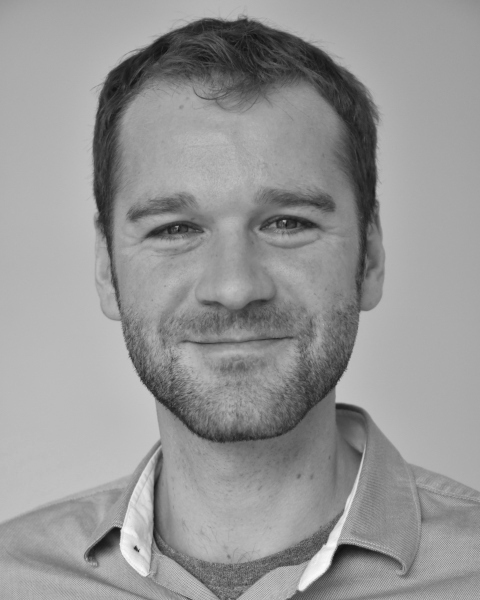
\includegraphics[width=1in,height=1.25in,clip,keepaspectratio]{./jpg/jmuenchow.jpg}}]{Jannes Muenchow}
	is a GIScientist working in tropical ecology since 2007 with a special interest in ENSO, biodiversity, species distribution modeling and predictive mapping.
	He has earned his PhD at the Friedrich-Alexander University Erlangen-Nuremberg (Germany) in 2013.
	He joined the business location department of a large consulting company as a geo-data scientist for more than two years until the prediction of a strong El Niño event brought him back to academia in 2016 (Friedrich Schiller University Jena).
	Currently, his research focuses on developing open source tools for ecology, geomorphology and qualitative GIS.
	He is a co-author of the book "Geocomputation with R".
\end{IEEEbiography}
\begin{IEEEbiography}
	[{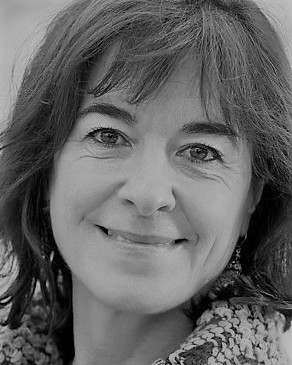
\includegraphics[width=1in,height=1.25in,clip,keepaspectratio]{./jpg/eiturritxa.jpg}}]{Eugenia Iturritxa}
	received the Ecology and Ph.D degree in Plant Protection from the Basque country University in 2001.
	Since 1999 her main research has focused on forest health, on the study of diverse species of native and introduced pathogenic fungi in forests and forest plantations.
	Her research includes the distribution of diseases, analysis of predisposing factors for them, genetic and phenotypic studies of populations and their epidemiology.
\end{IEEEbiography}
\begin{IEEEbiography}
	[{
\includegraphics[width=1in,height=1.25in,clip,keepaspectratio]{./jpg/jcortes.png}}]{José Cortés}
	received his B.S. in Mathematics and M.S. in Statistics from Arizona State University, Arizona, USA, in 2014 and 2016, respectively.
	Currently he is a PhD student at Friedrich-Schiller-University, Jena, Germany.
	He is a member of the International Max Planck Research School on Global Biogeochemical Cycles (IMPRS-gBGC), a joint program with the Max Planck Institute for Biogeochemistry.
	His research focuses on spatio-temporal trend detection in environmental data.
\end{IEEEbiography}
\begin{IEEEbiography}
	[{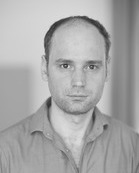
\includegraphics[width=1in,height=1.25in,clip,keepaspectratio]{./jpg/bbischl.jpg}}]{Bernd Bischl}
	obtained his Ph.D from Dortmund Technical University in 2013.
	He is a professor for "Statistical Learning and Data Science" at the Department of Statistics at the Ludwig-Maximilians-University Munich and a director of the "Munich Center for Machine Learning".
	His research interests include AutoML, model selection, interpretable ML and XAI.
\end{IEEEbiography}
\begin{IEEEbiography}
	[{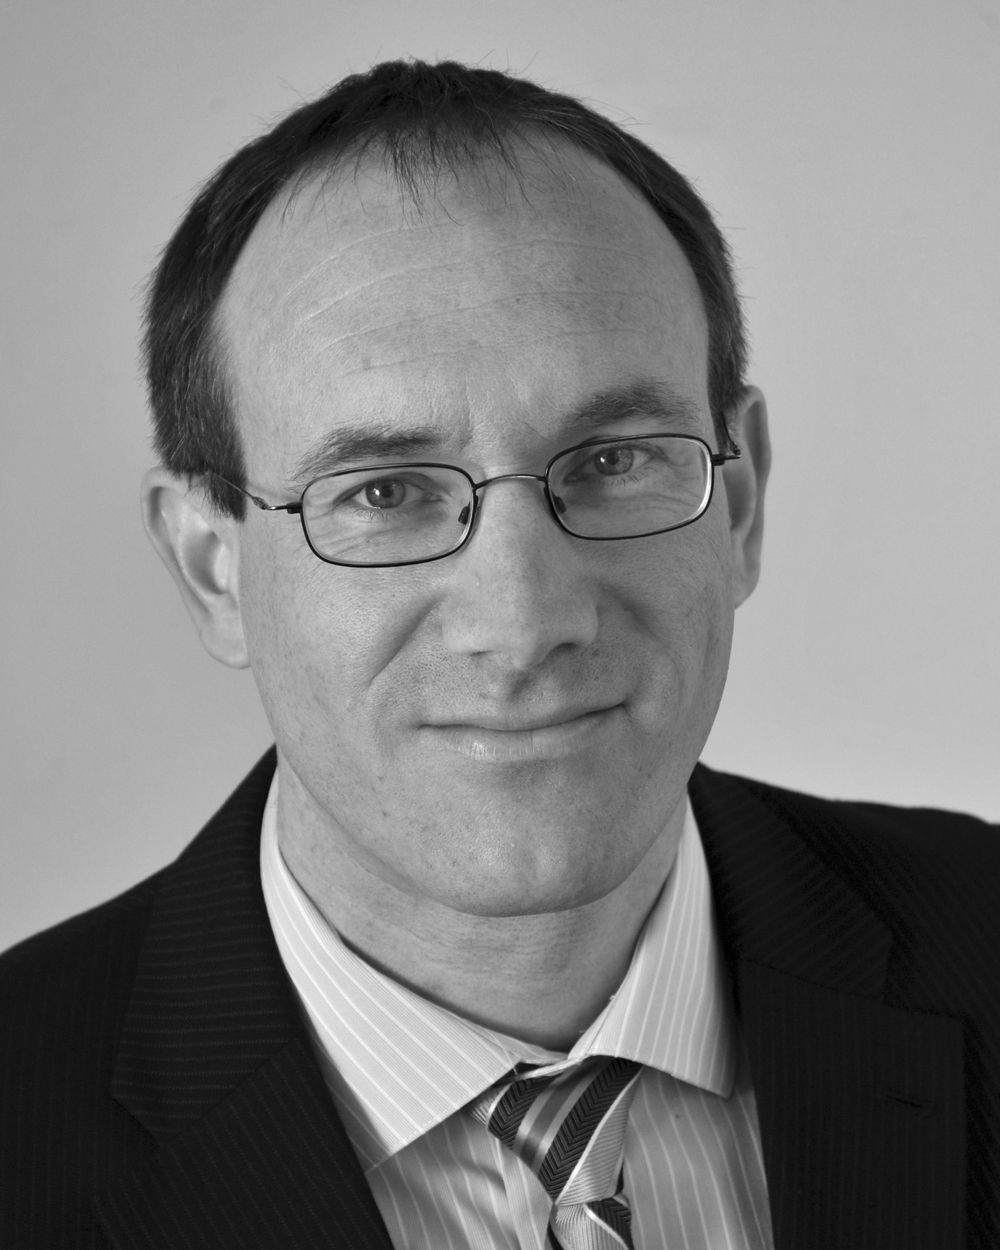
\includegraphics[width=1in,height=1.25in,clip,keepaspectratio]{./jpg/abrenning.jpg}}]{Alexander Brenning}
	(Ph.D. 2005) graduated in mathematics at Technical University of Freiberg, Germany, and received his Ph.D. in geography from Humboldt-Universität zu Berlin.
	He served as an assistant professor and tenured associate professor in geomatics at the University from 2007 until 2015, when he was appointed as a full professor in geographic information science at Friedrich Schiller University Jena, Germany.
	Dr. Brenning's research interests include statistical and machine-learning techniques for environmental modeling and remote sensing.
	He has also contributed to open-source geocomputation by developing R packages for spatial cross-validation and GIS coupling.
\end{IEEEbiography}

\end{document}
